\section{Messergebnisse und Auswertung}

\subsection{Vorgehensweise bei der Auswertung}
Beispiel: R1
\begin{figure}[H]
\begin{center}
  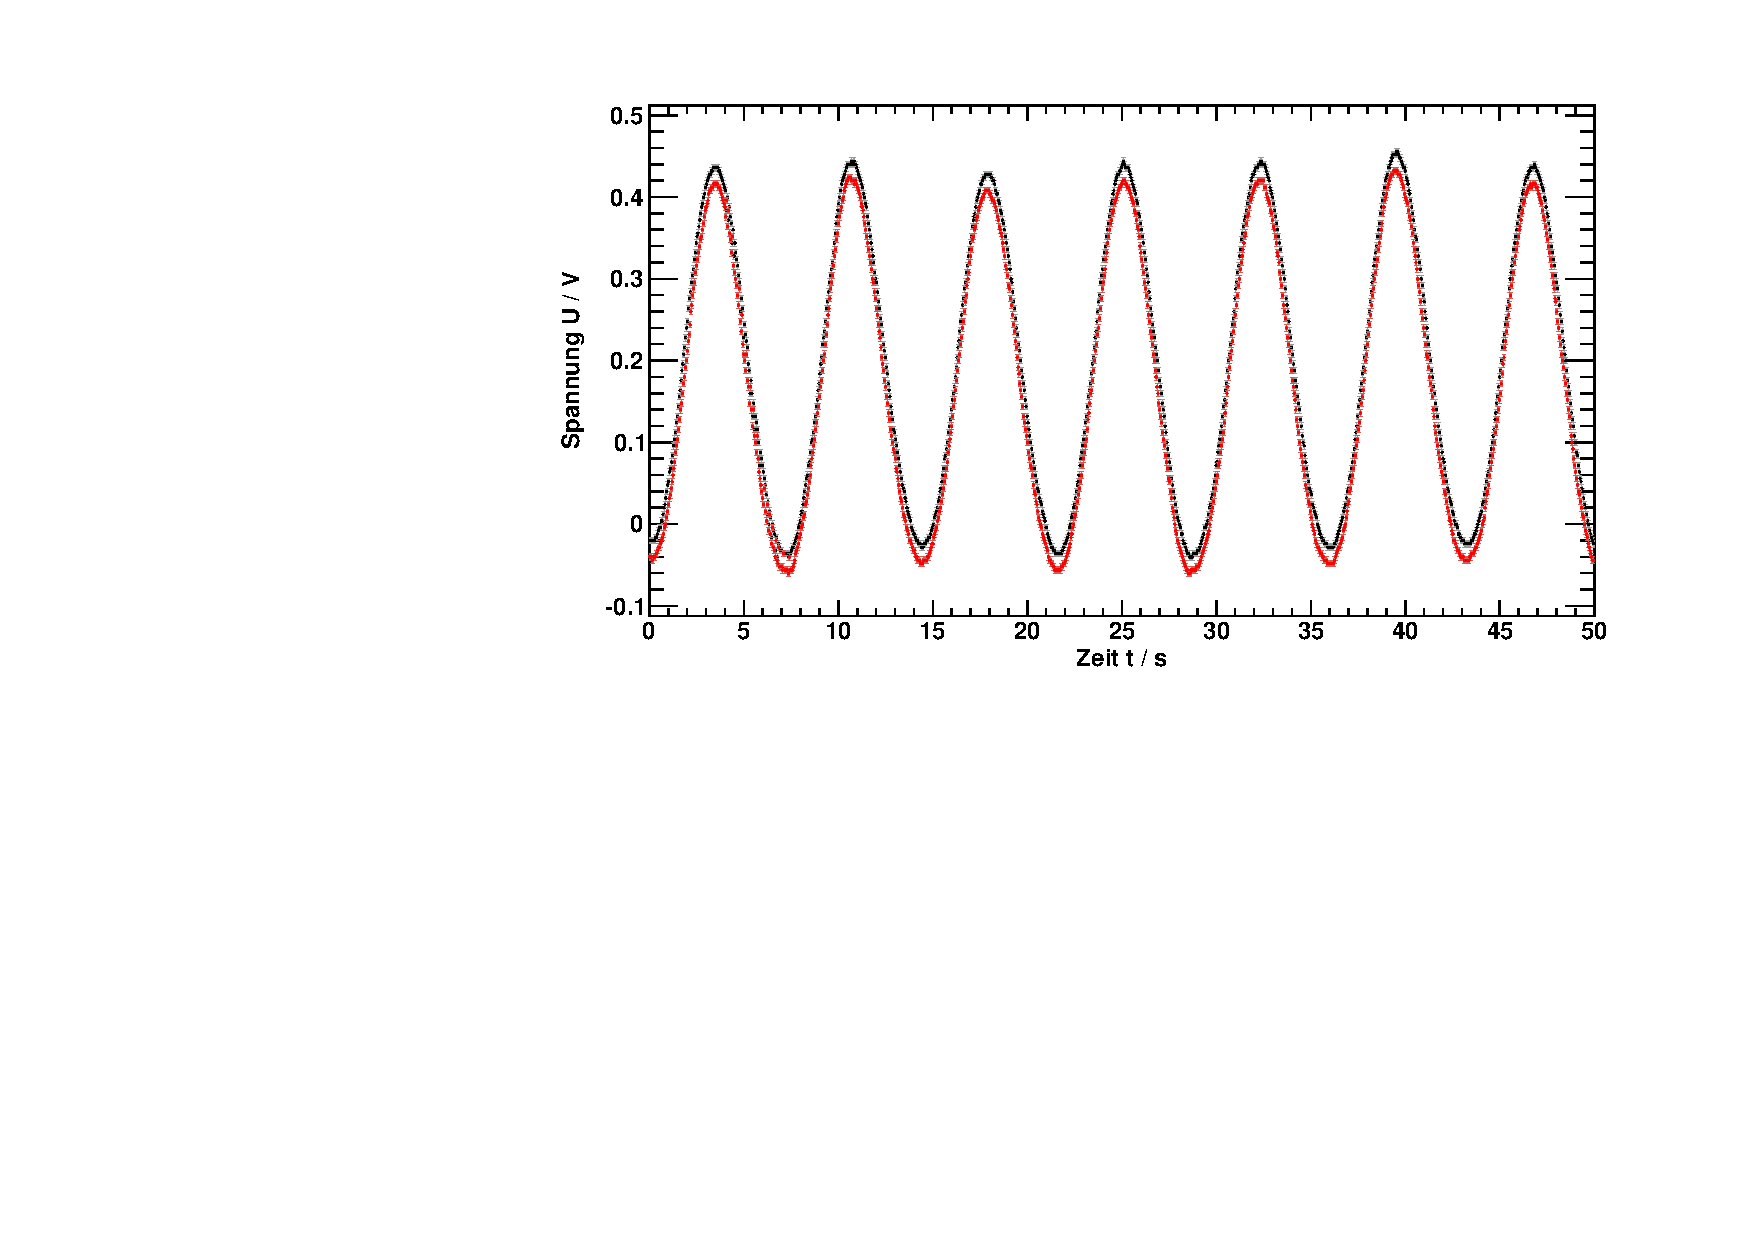
\includegraphics[width=\textwidth]{../img/both_Spule_R1.pdf}
  \caption{caption}
  \label{img:ex:both}
\end{center}
\end{figure}

\begin{figure}[H]
\begin{center}
  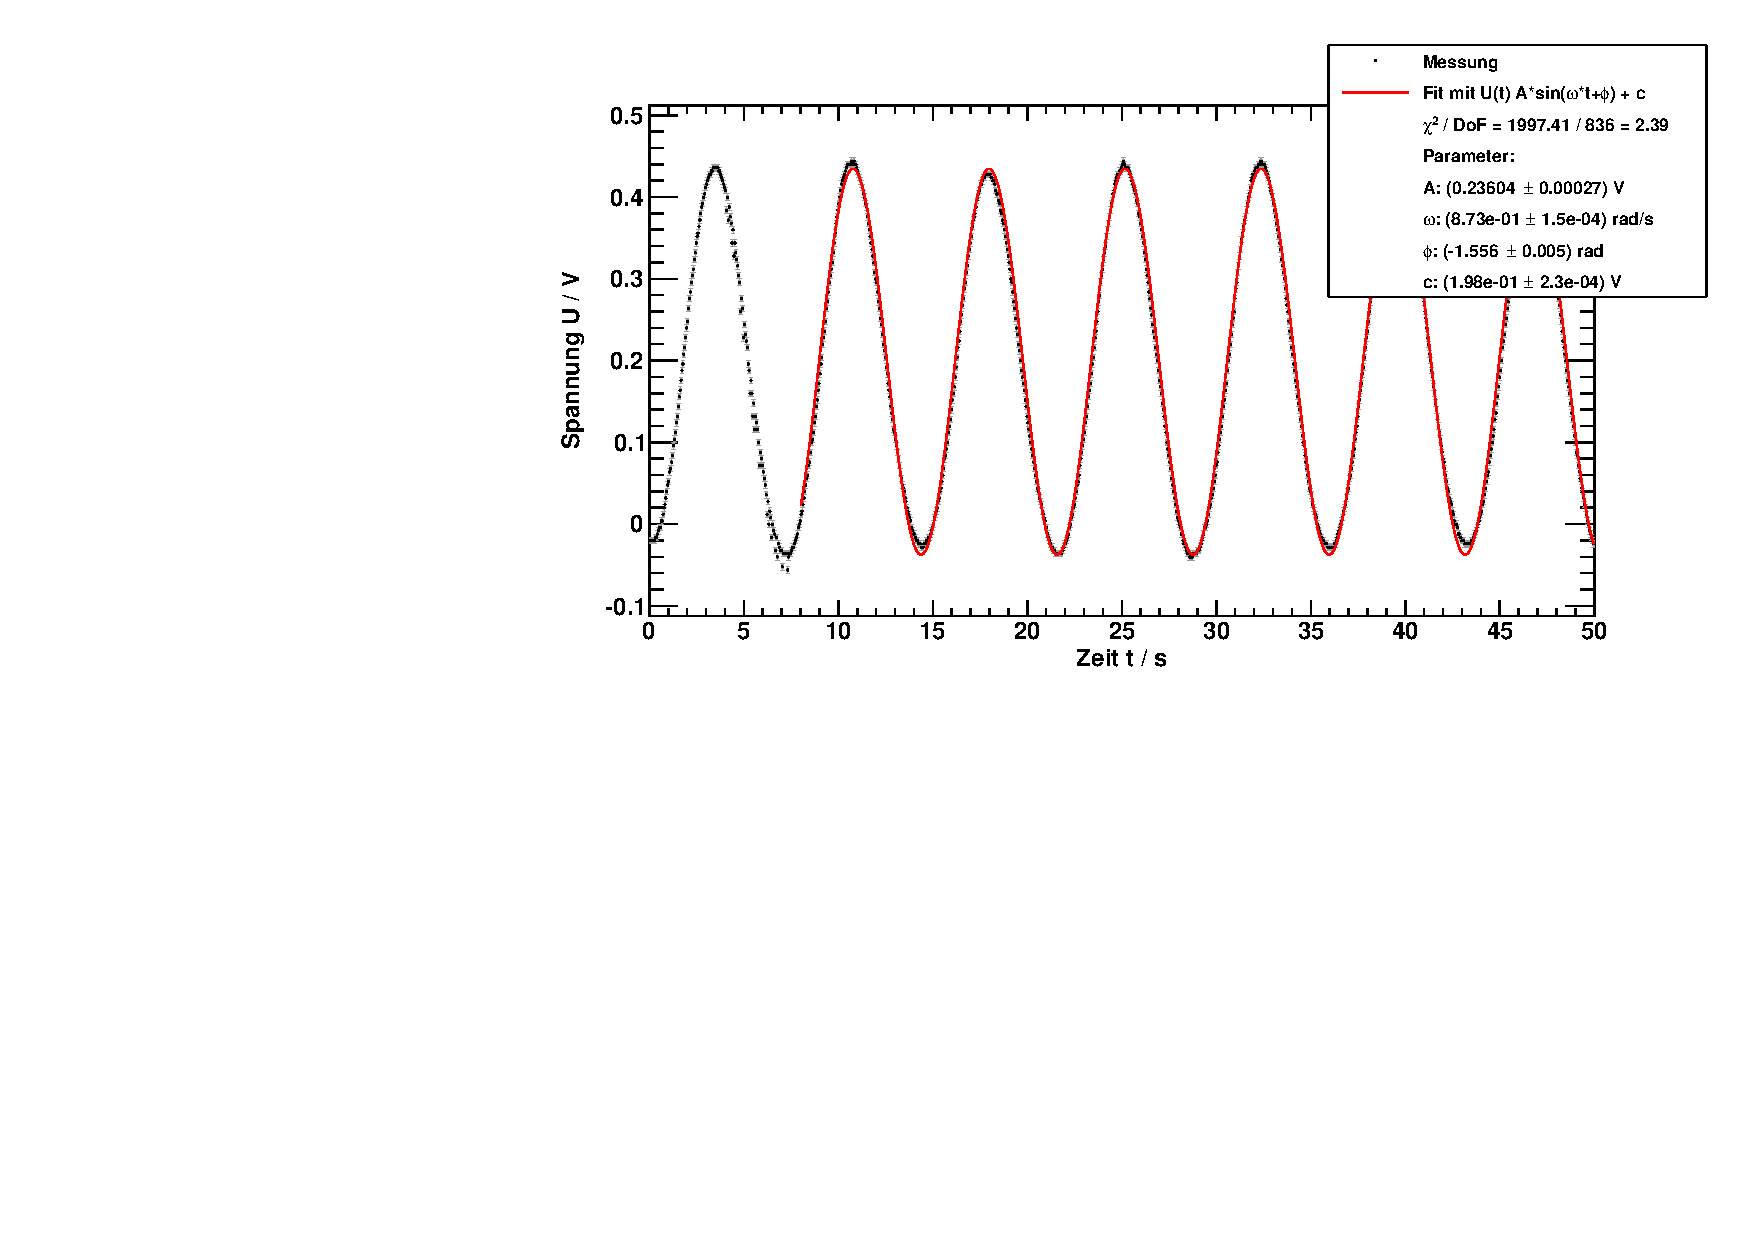
\includegraphics[width=\textwidth]{../img/fit_Spule_R1.pdf}
  \caption{caption}
  \label{img:ex:fit}
\end{center}
\end{figure}
\begin{figure}[H]
\begin{center}
  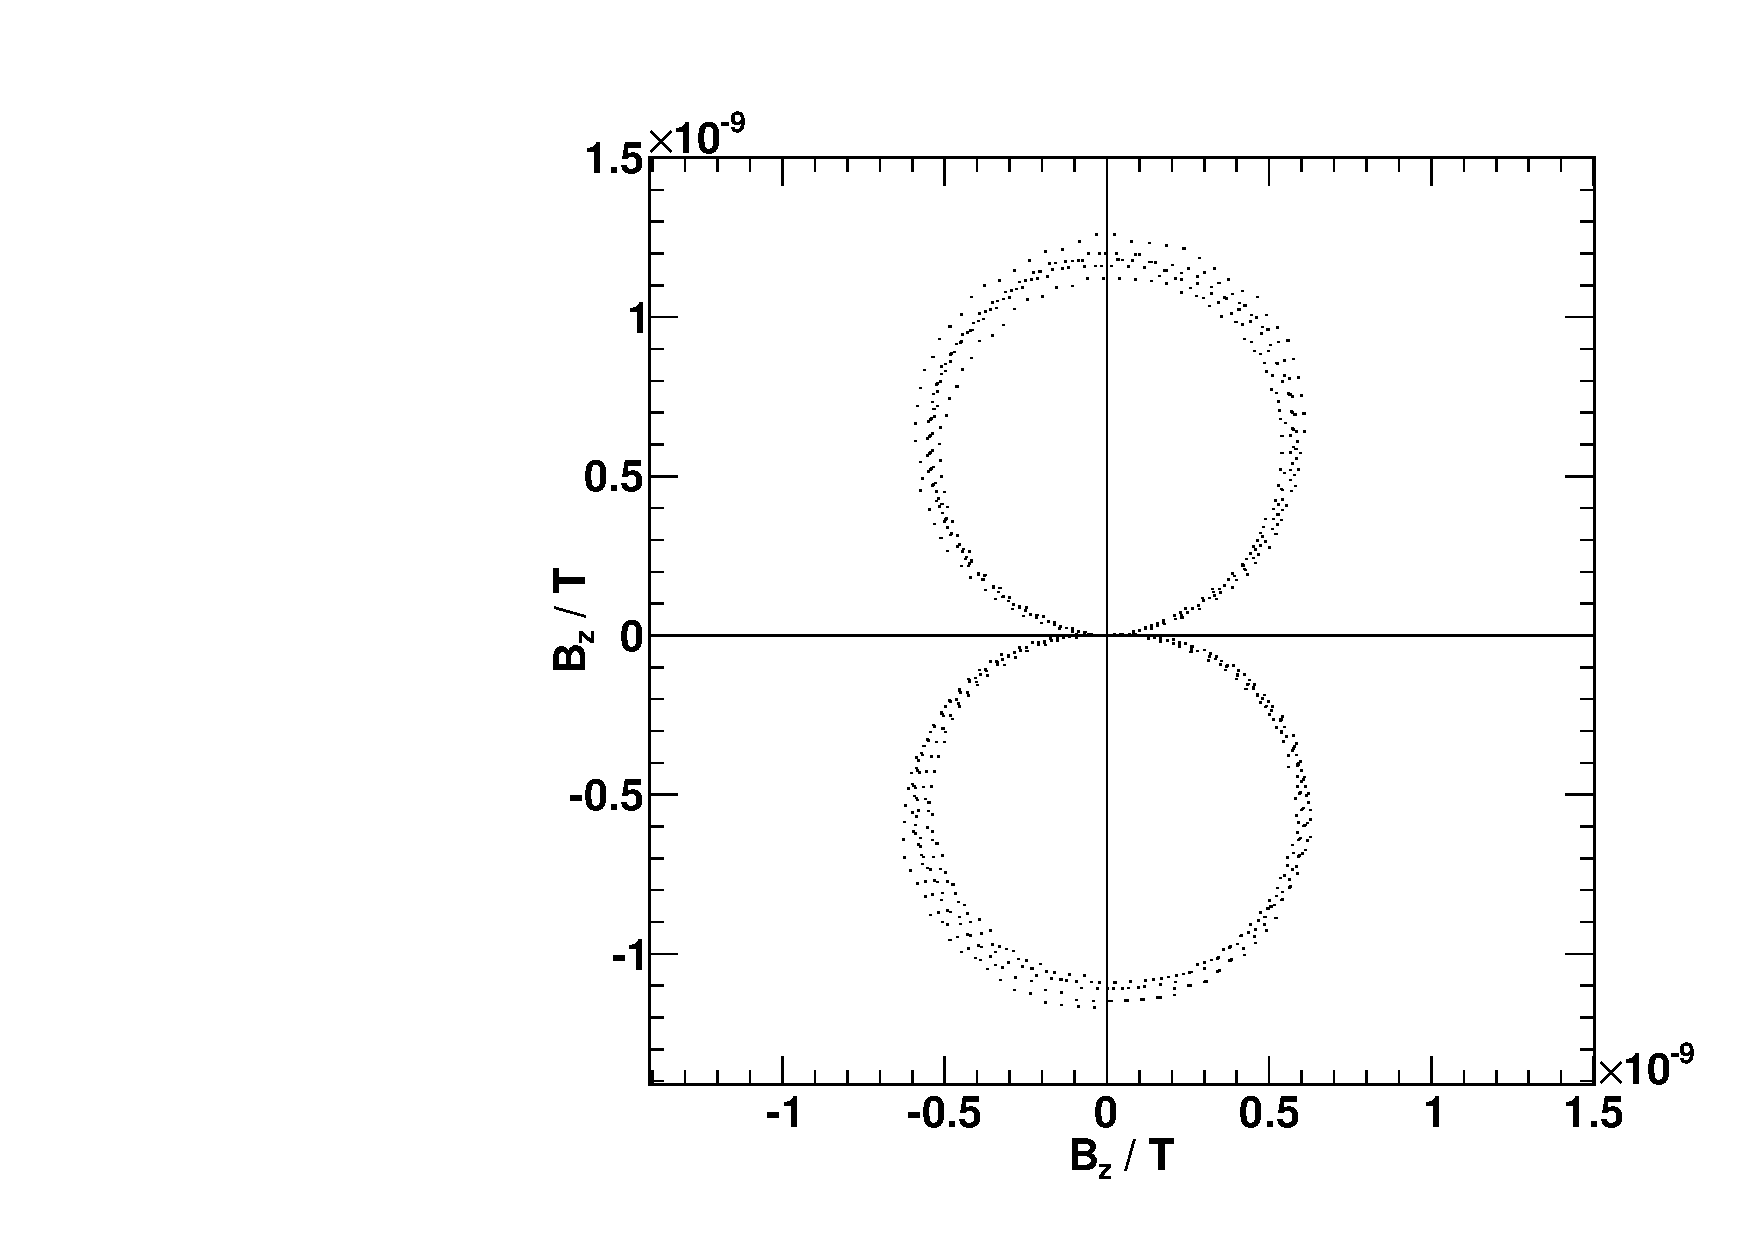
\includegraphics[width=0.5\textwidth]{../img/polar_Spule_R1.pdf}
  \caption{caption}
  \label{img:ex:polar}
\end{center}
\end{figure}

\subsection{Vermessung des Magnetfeldes der Leiterschleife}
\subsubsection{Berechnung aus der SQUID-Messung}
\begin{figure}[H]
\begin{center}
  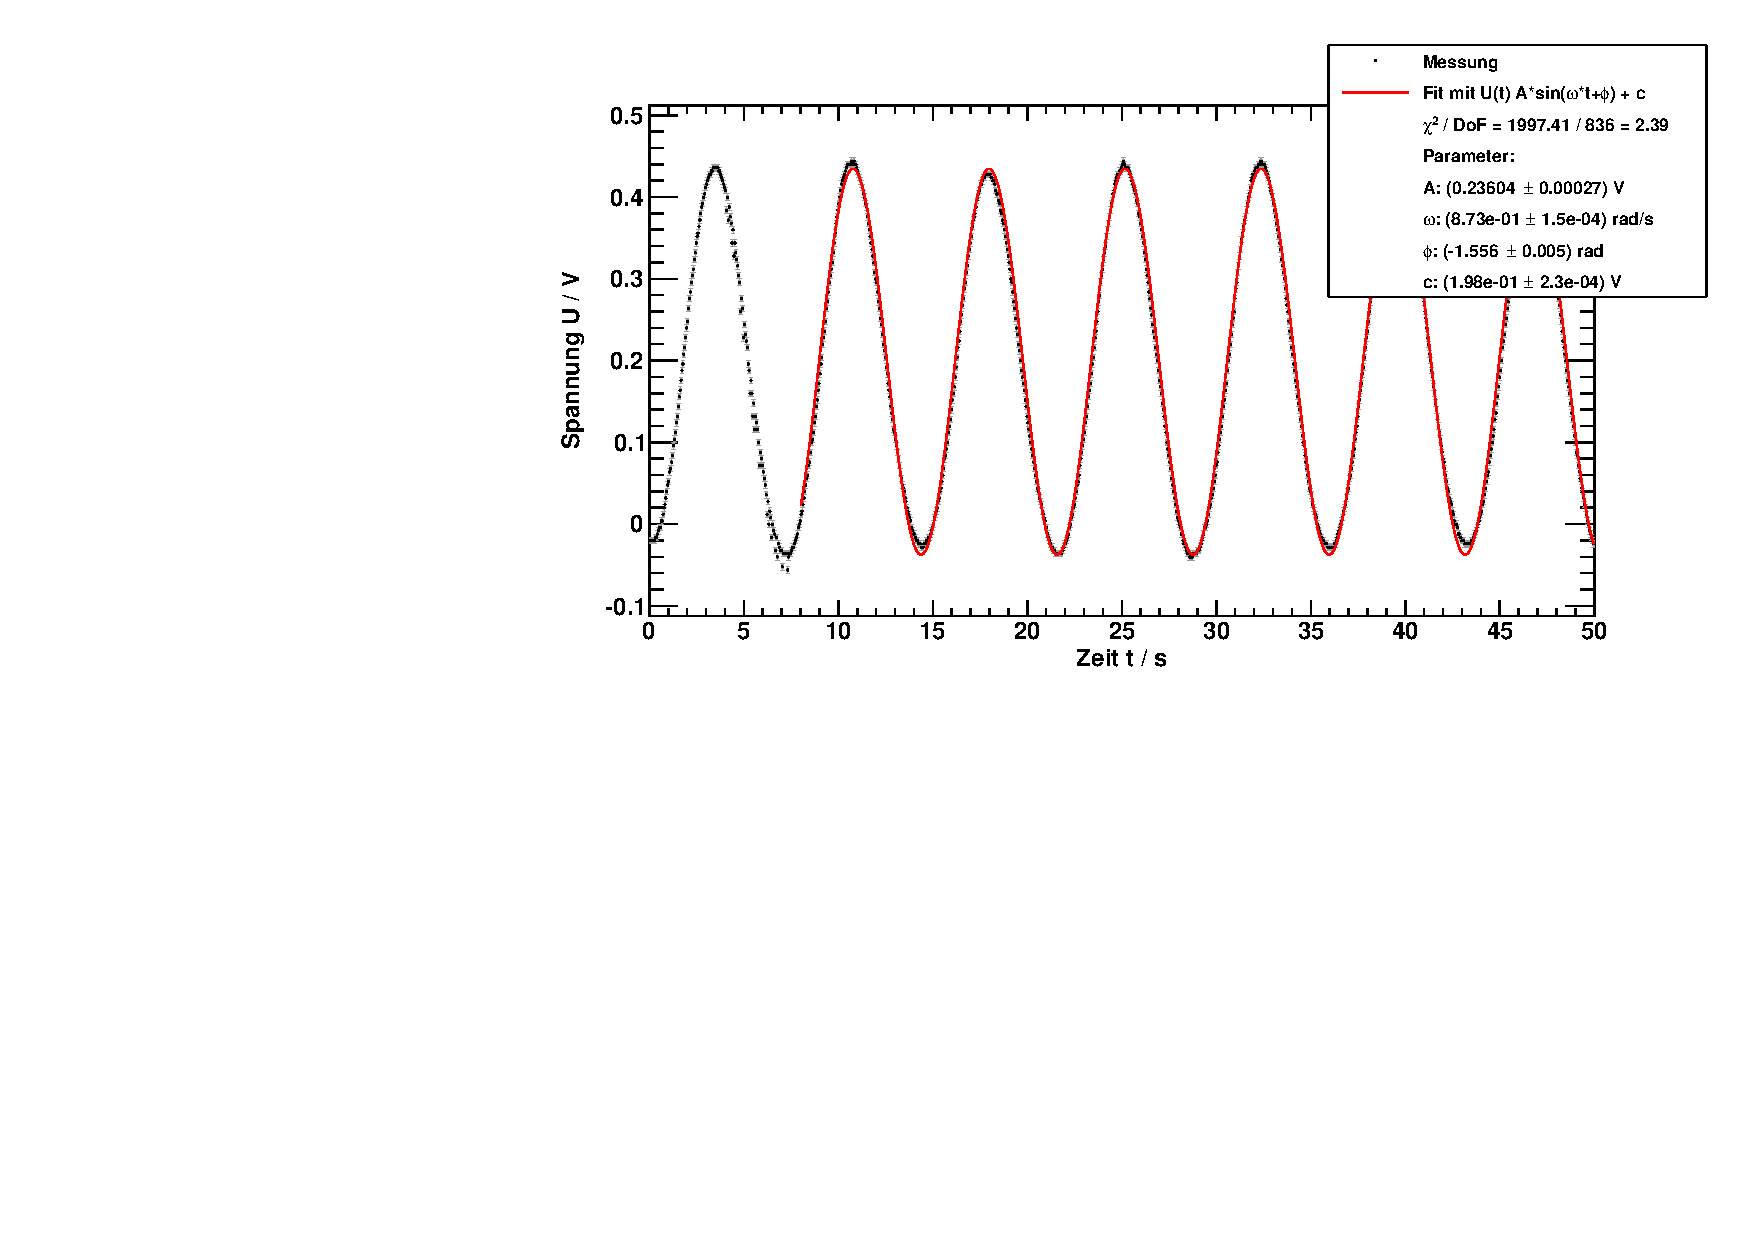
\includegraphics[width=0.64\textwidth]{../img/fit_Spule_R1.pdf}
  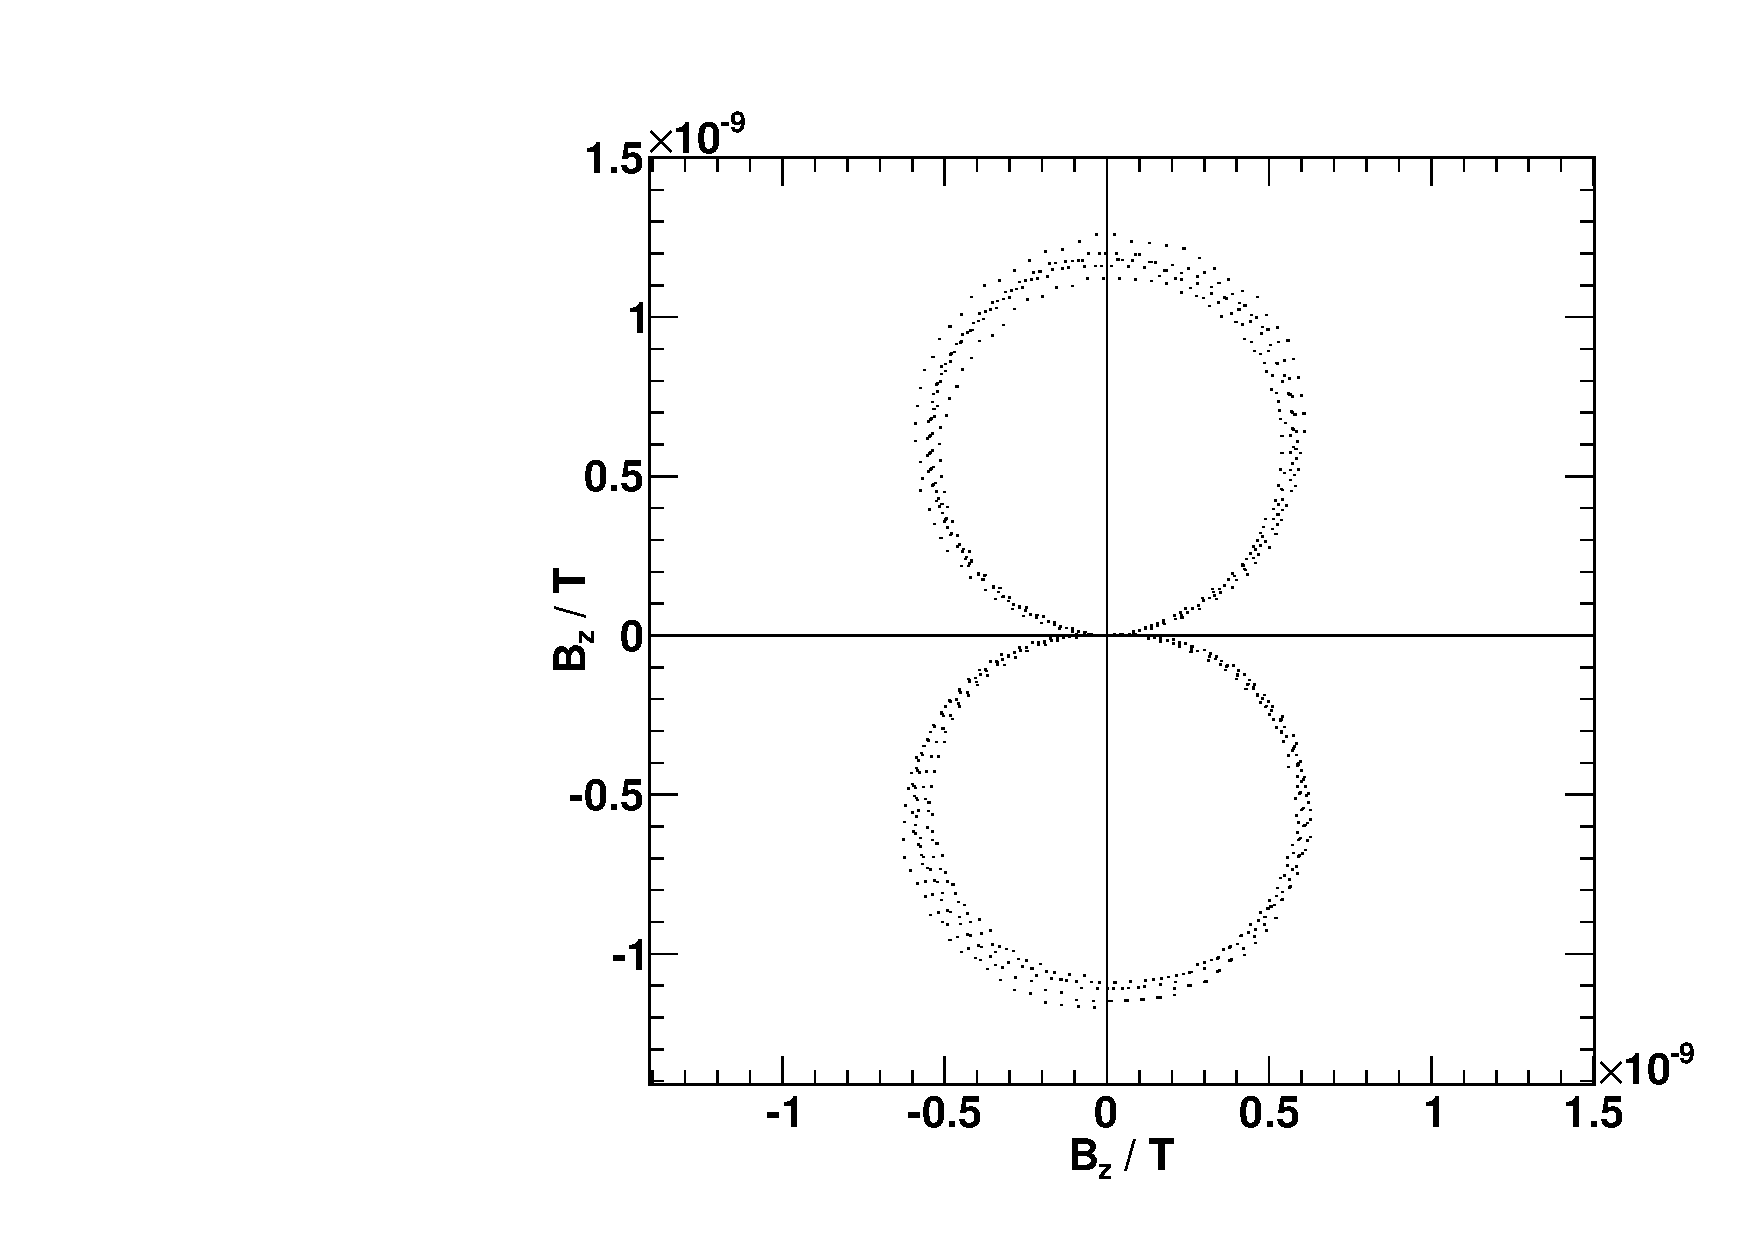
\includegraphics[width=0.35\textwidth]{../img/polar_Spule_R1.pdf}
  \caption{caption}
  \label{img:R1}
\end{center}
\end{figure}

\begin{figure}[H]
\begin{center}
  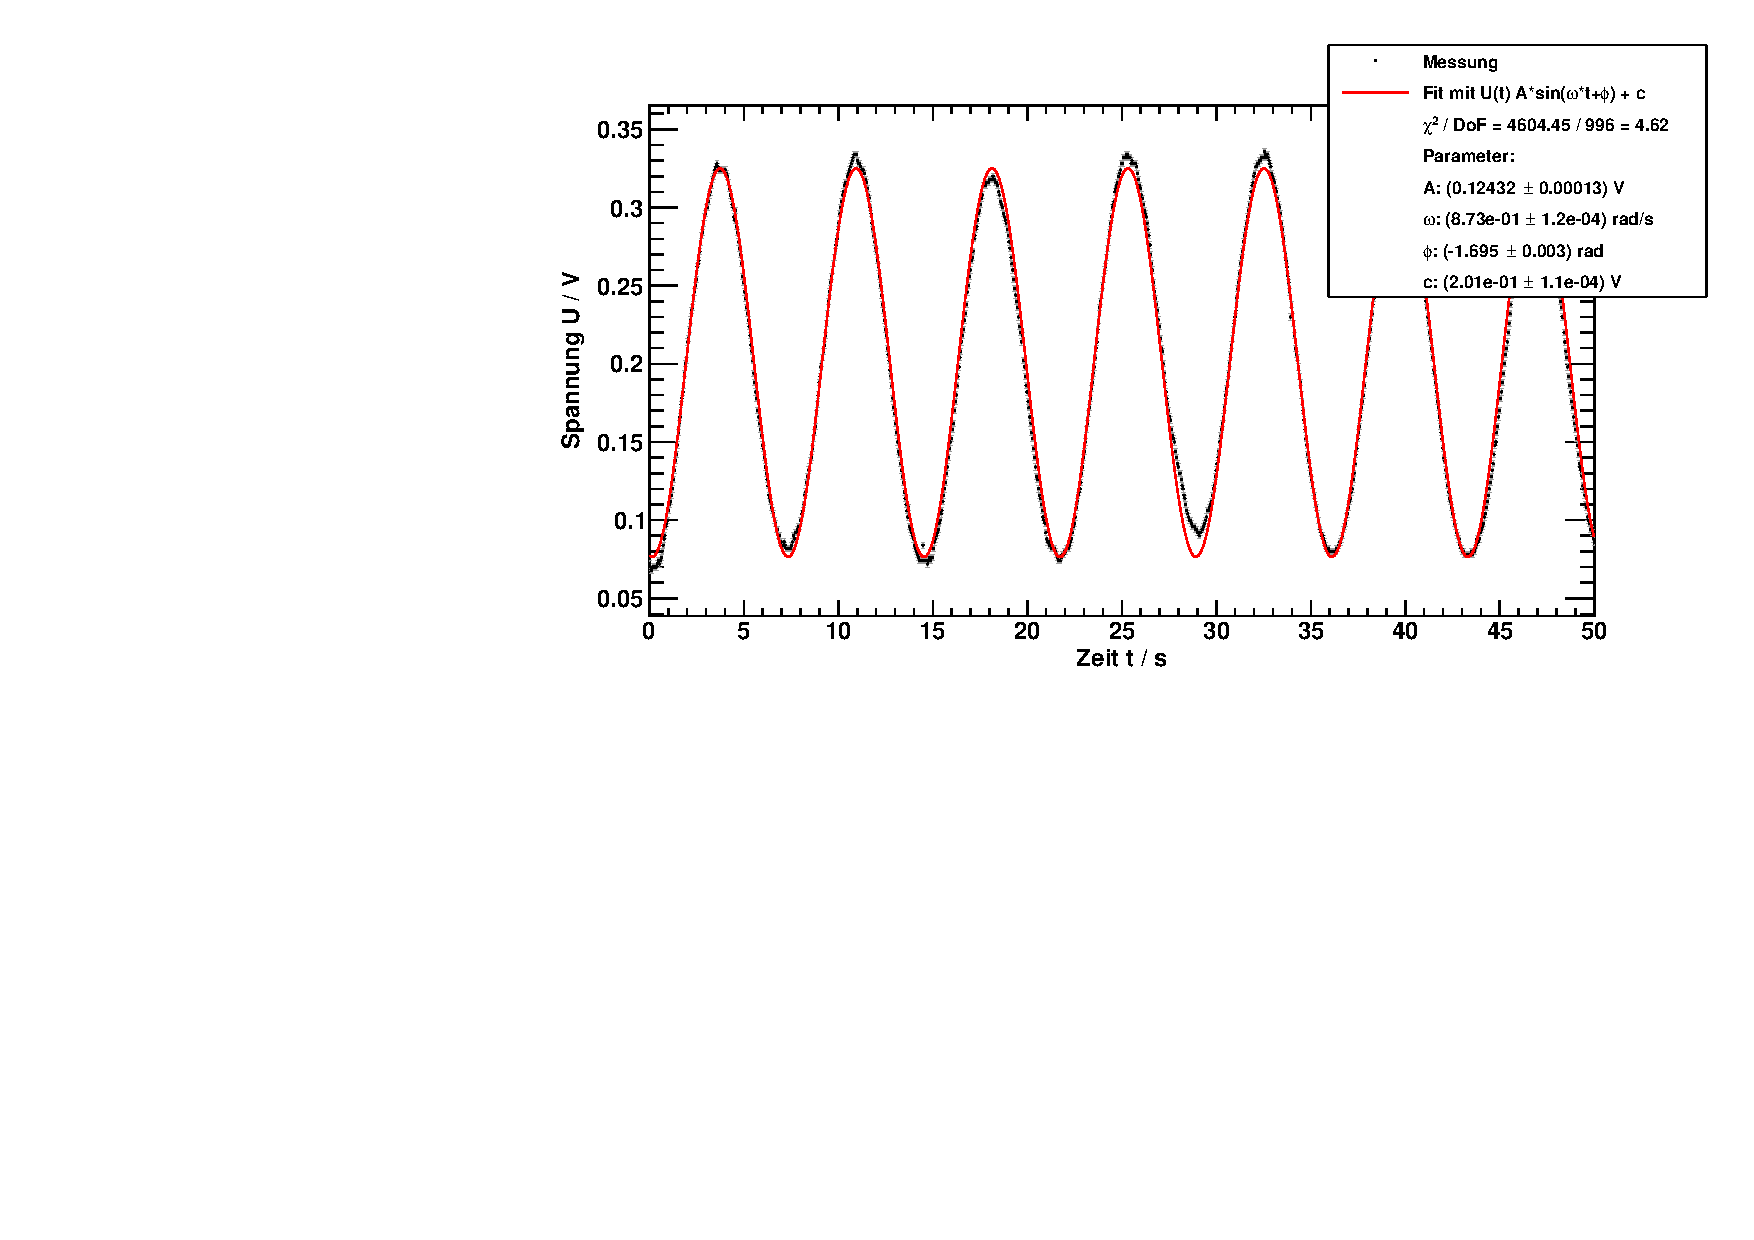
\includegraphics[width=0.64\textwidth]{../img/fit_Spule_R2.pdf}
  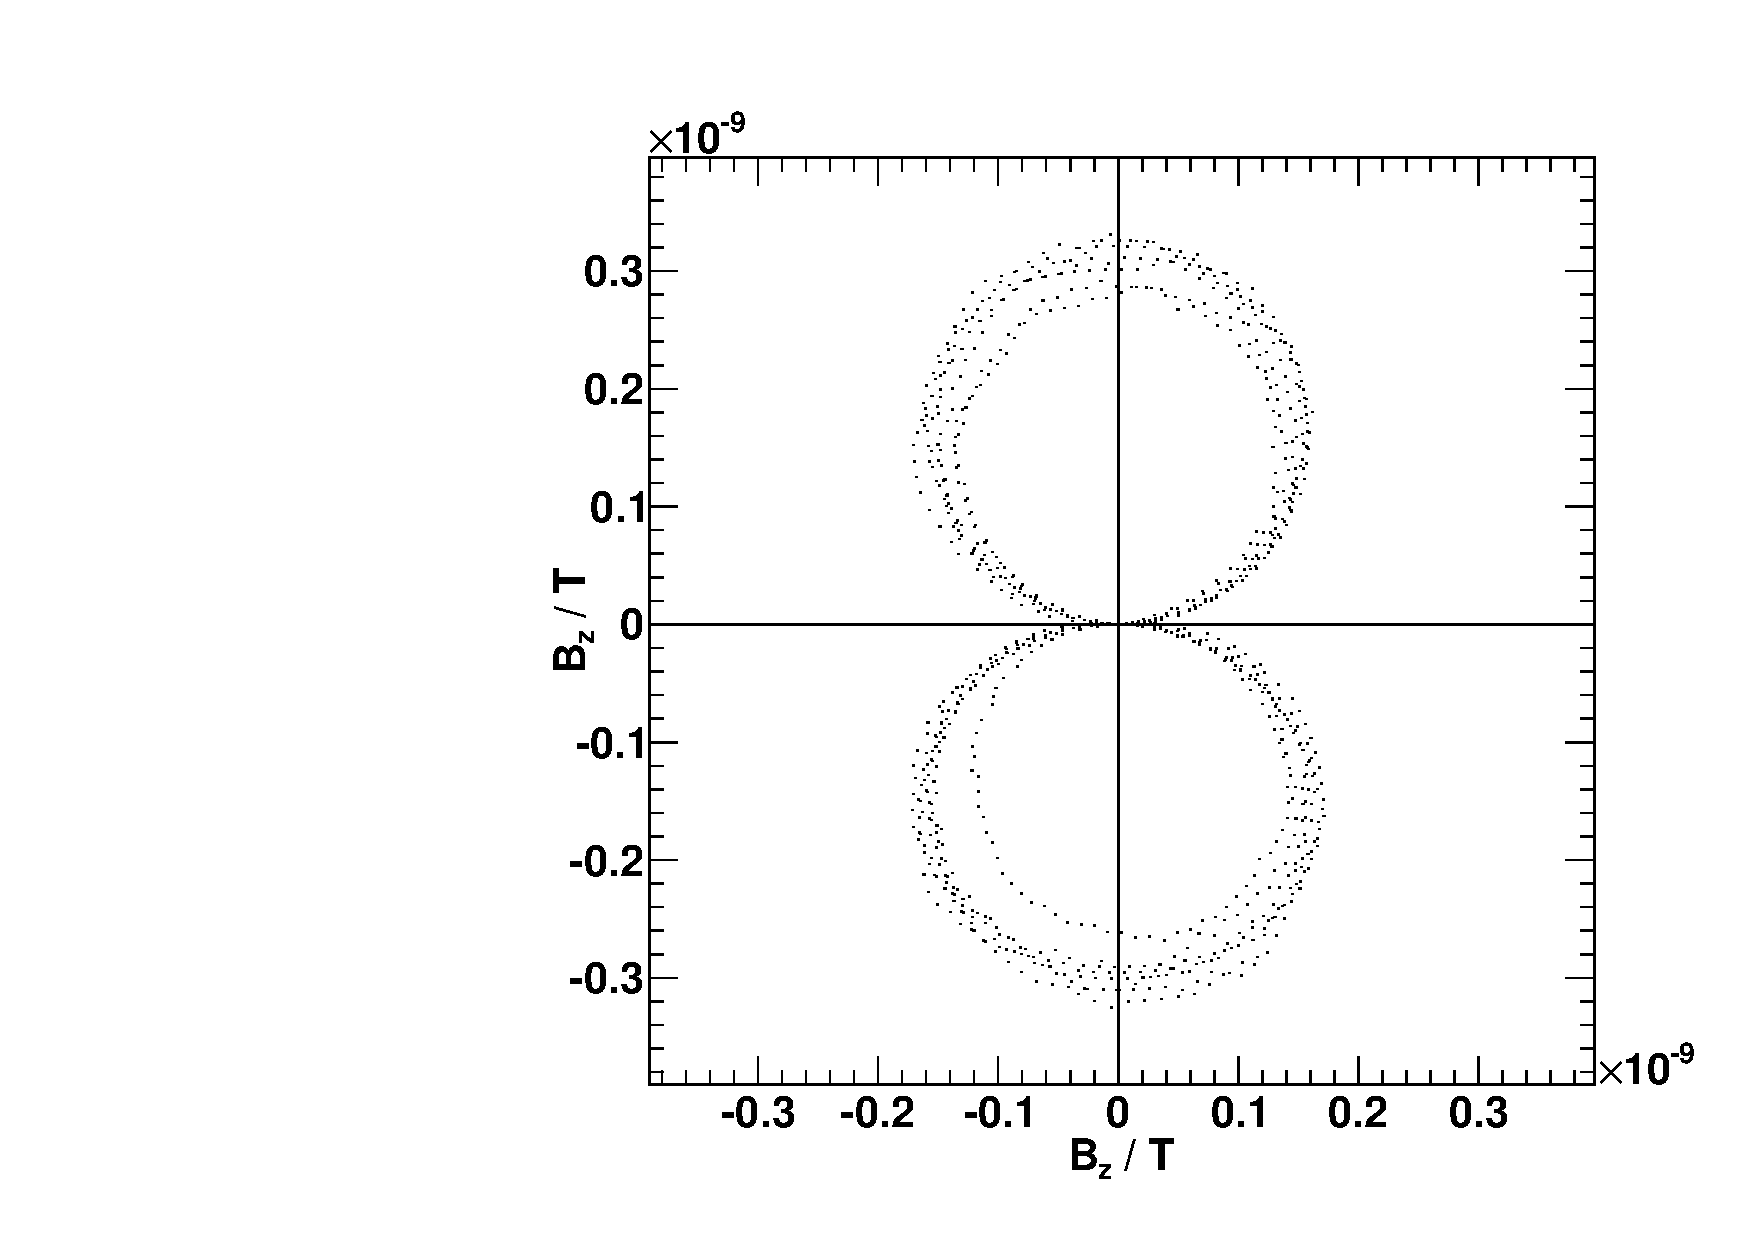
\includegraphics[width=0.35\textwidth]{../img/polar_Spule_R2.pdf}
  \caption{caption}
  \label{img:R2}
\end{center}
\end{figure}

\begin{figure}[H]
\begin{center}
  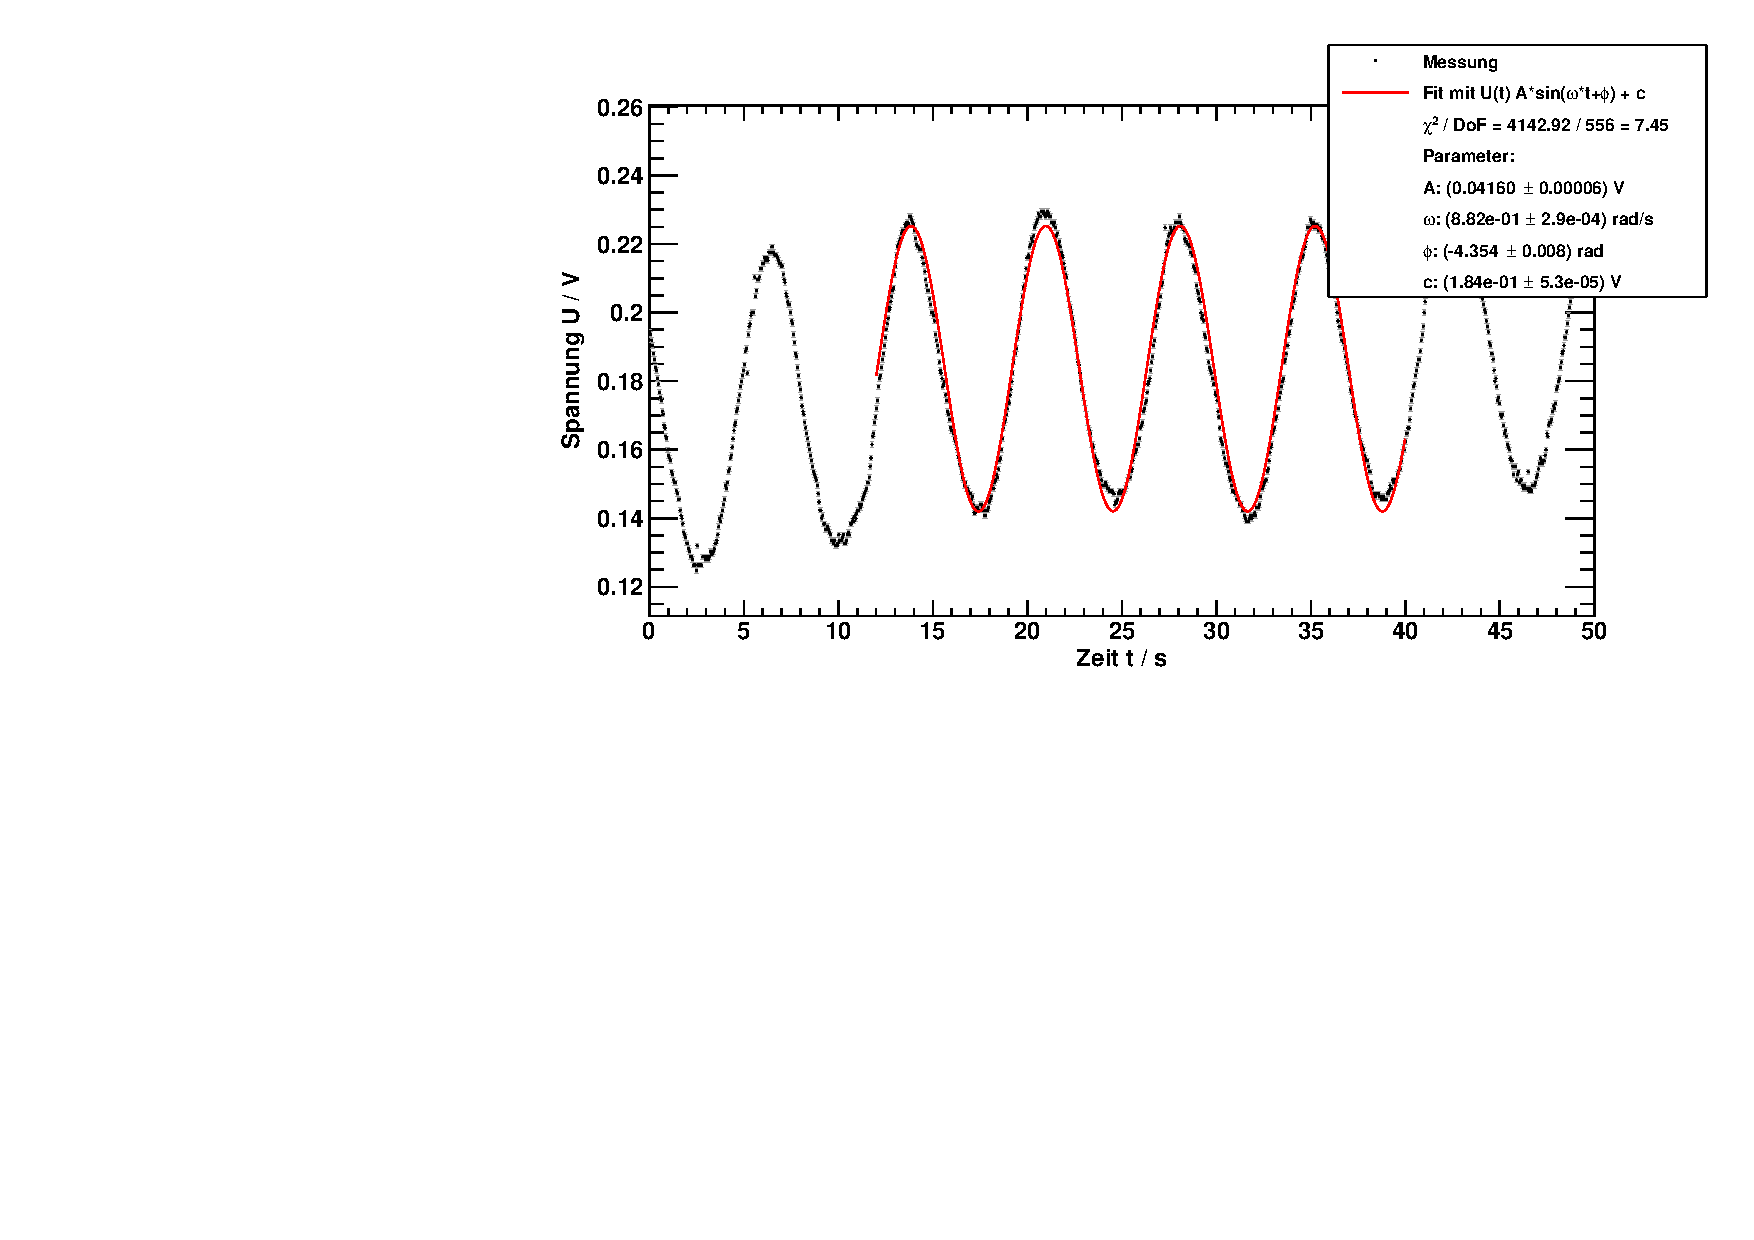
\includegraphics[width=0.64\textwidth]{../img/fit_Spule_R3.pdf}
  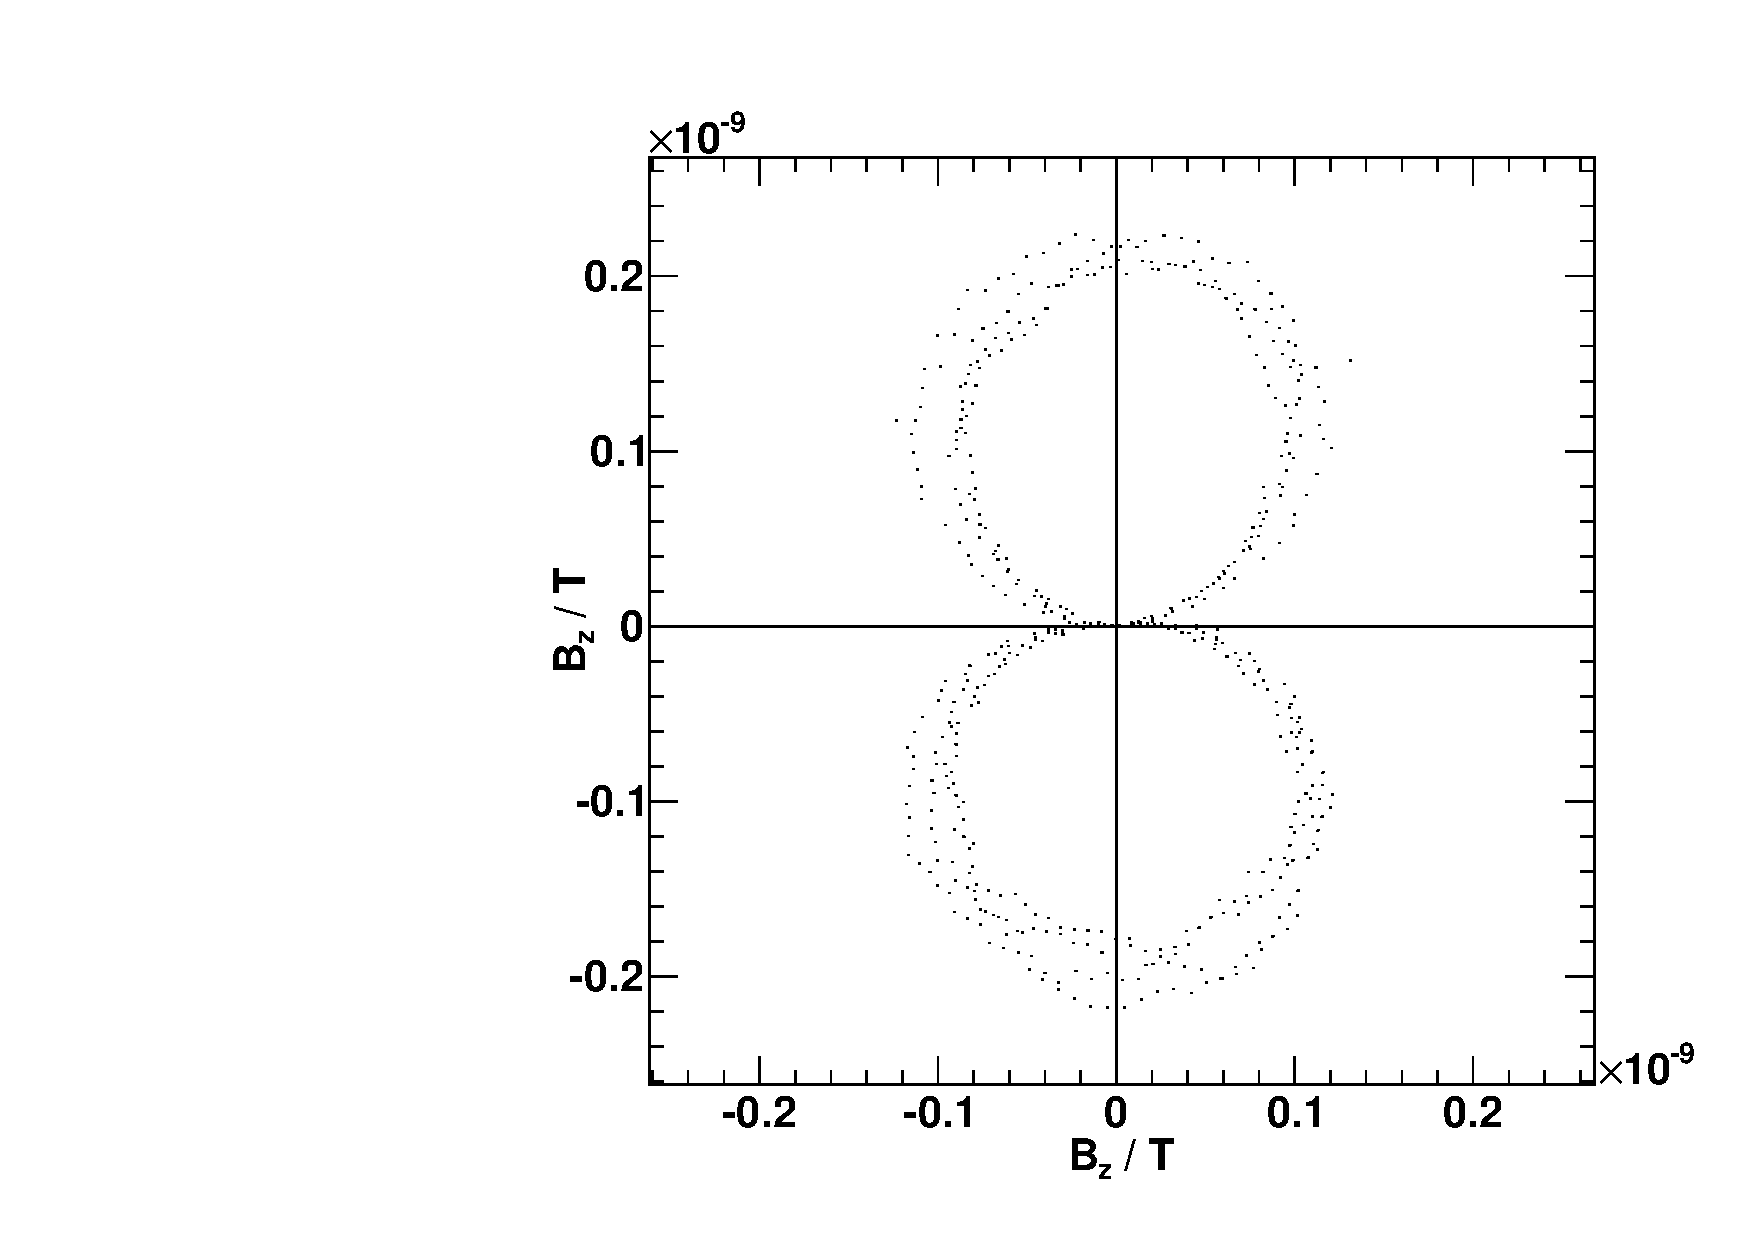
\includegraphics[width=0.35\textwidth]{../img/polar_Spule_R3.pdf}
  \caption{caption}
  \label{img:R3}
\end{center}
\end{figure}

\begin{figure}[H]
\begin{center}
  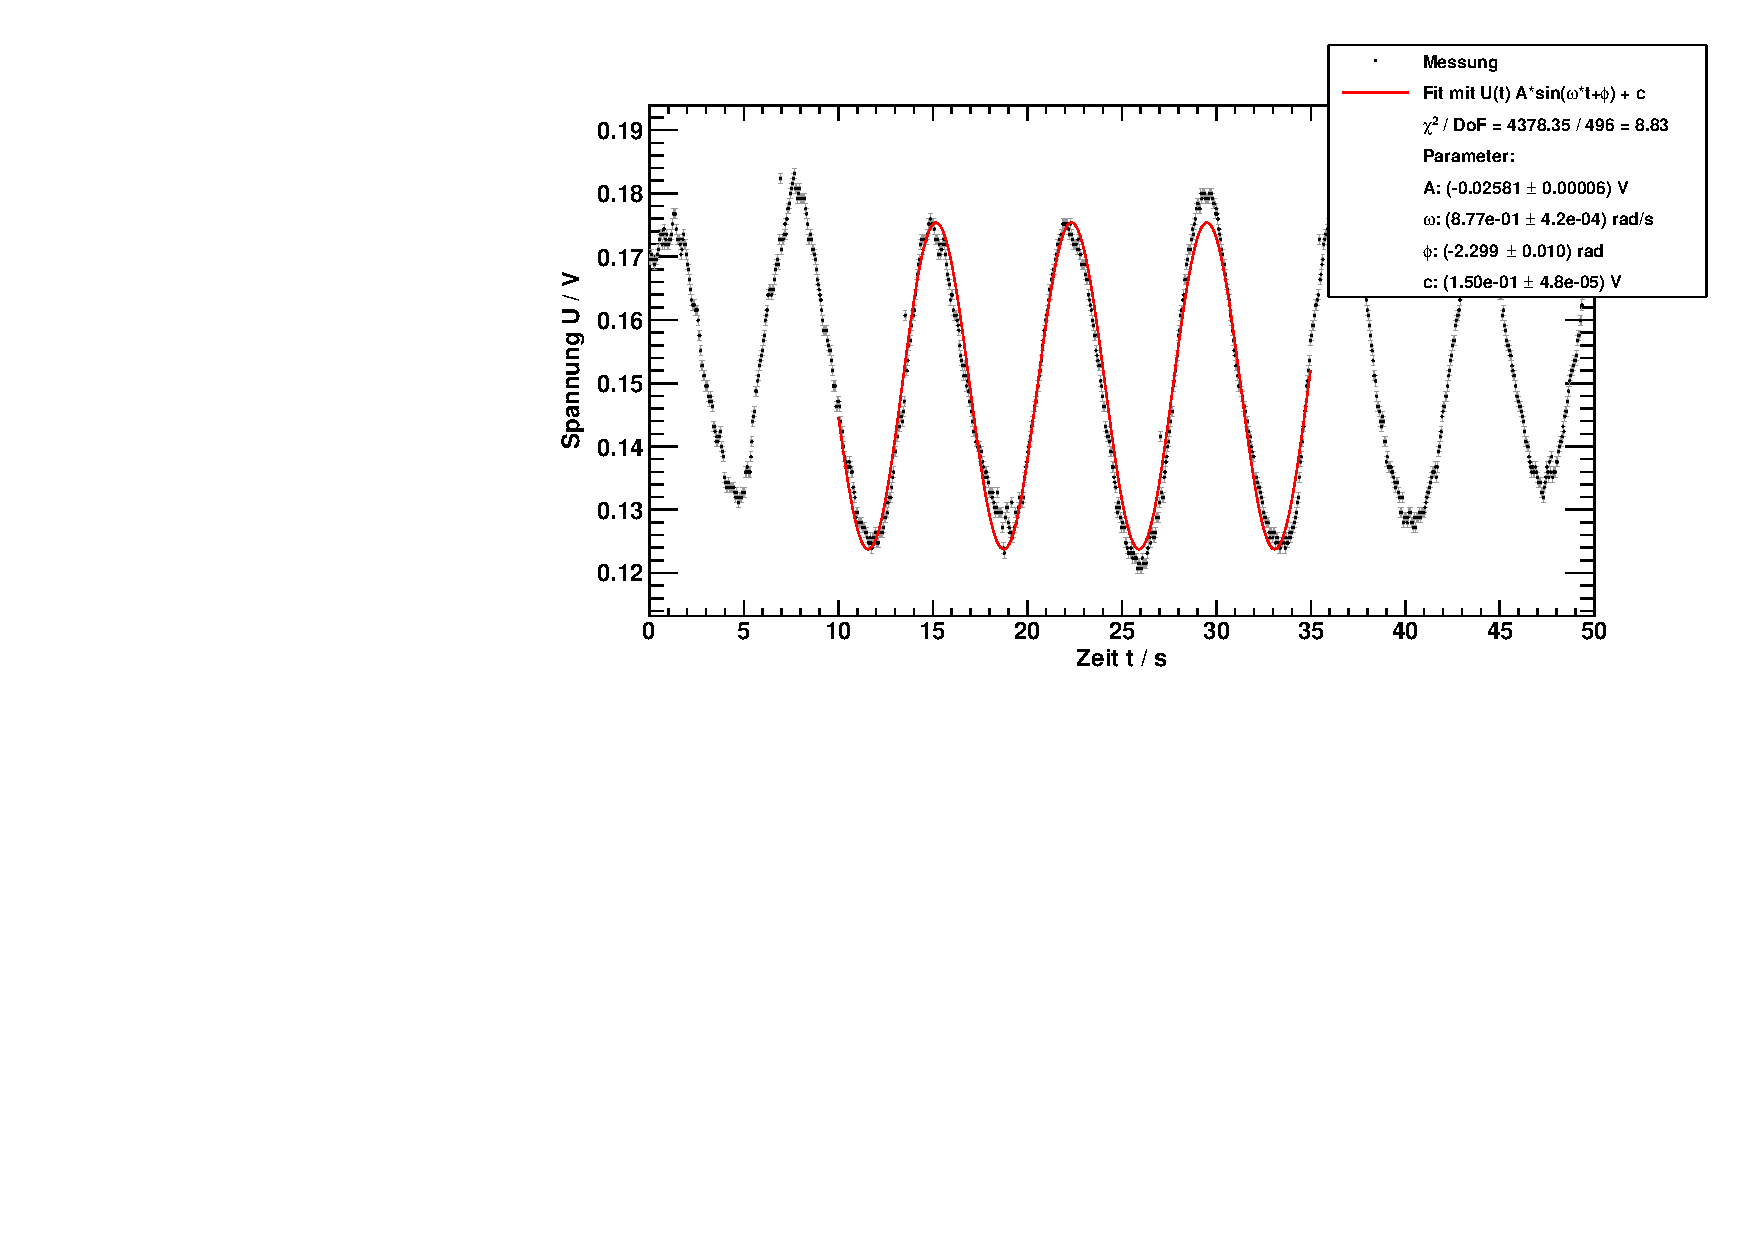
\includegraphics[width=0.64\textwidth]{../img/fit_Spule_R4.pdf}
  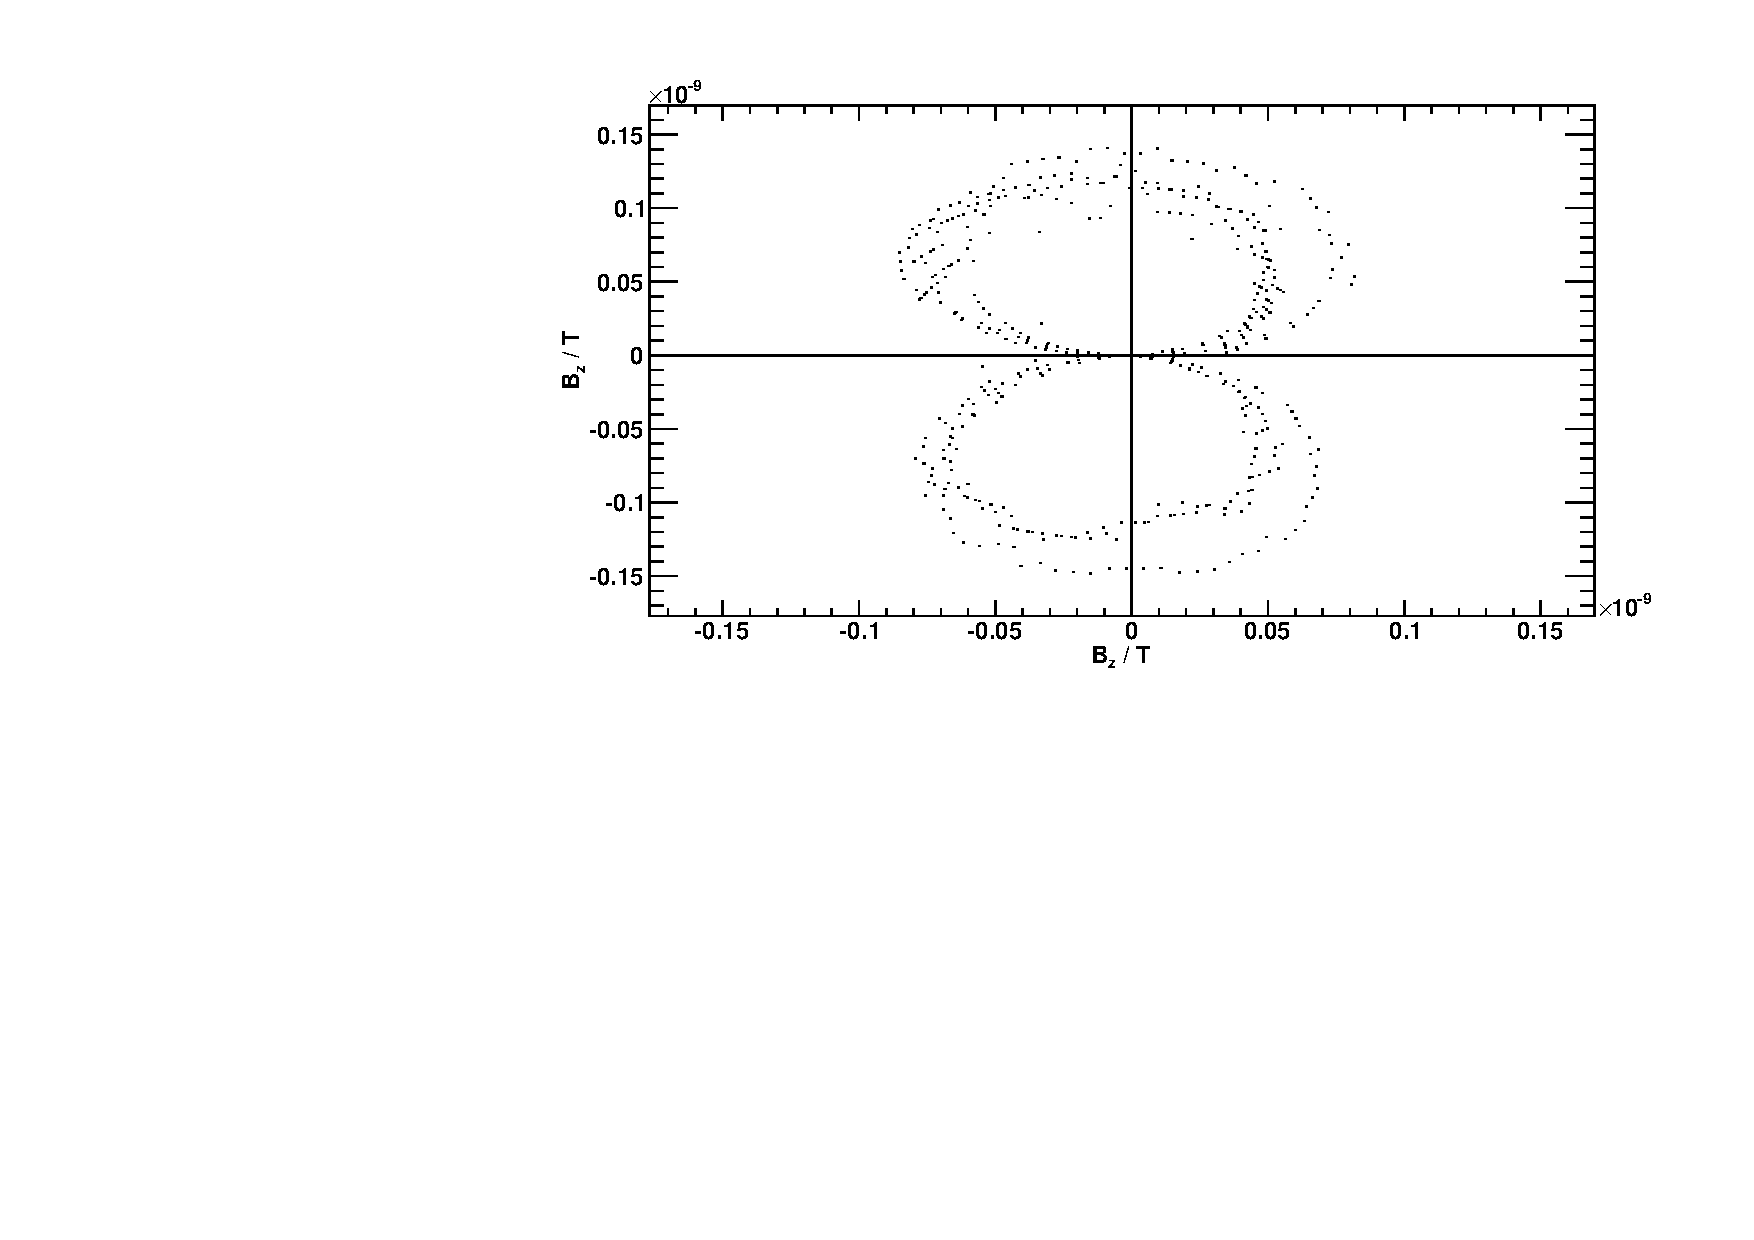
\includegraphics[width=0.35\textwidth]{../img/polar_Spule_R4.pdf}
  \caption{caption}
  \label{img:R4}
\end{center}
\end{figure}

\begin{figure}[H]
\begin{center}
  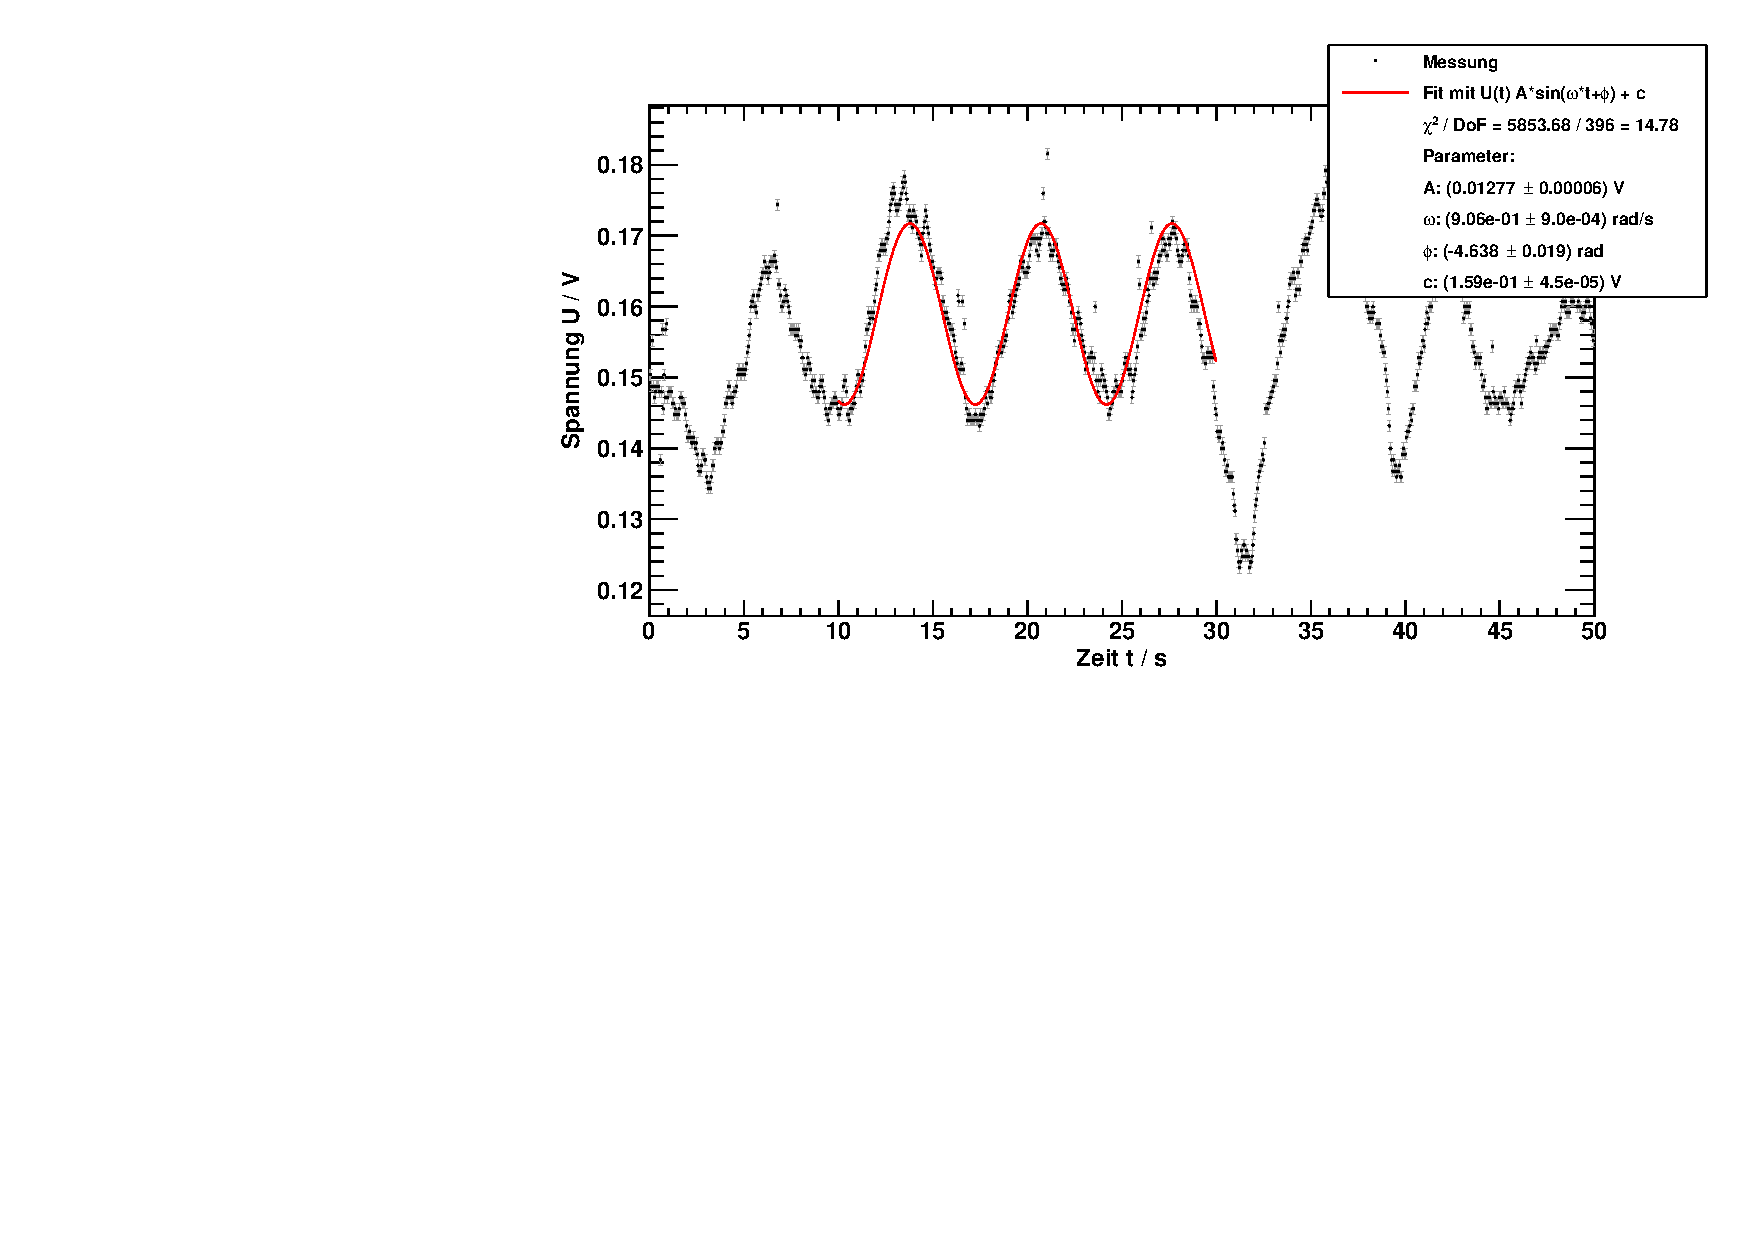
\includegraphics[width=0.64\textwidth]{../img/fit_Spule_R5_1.pdf}
  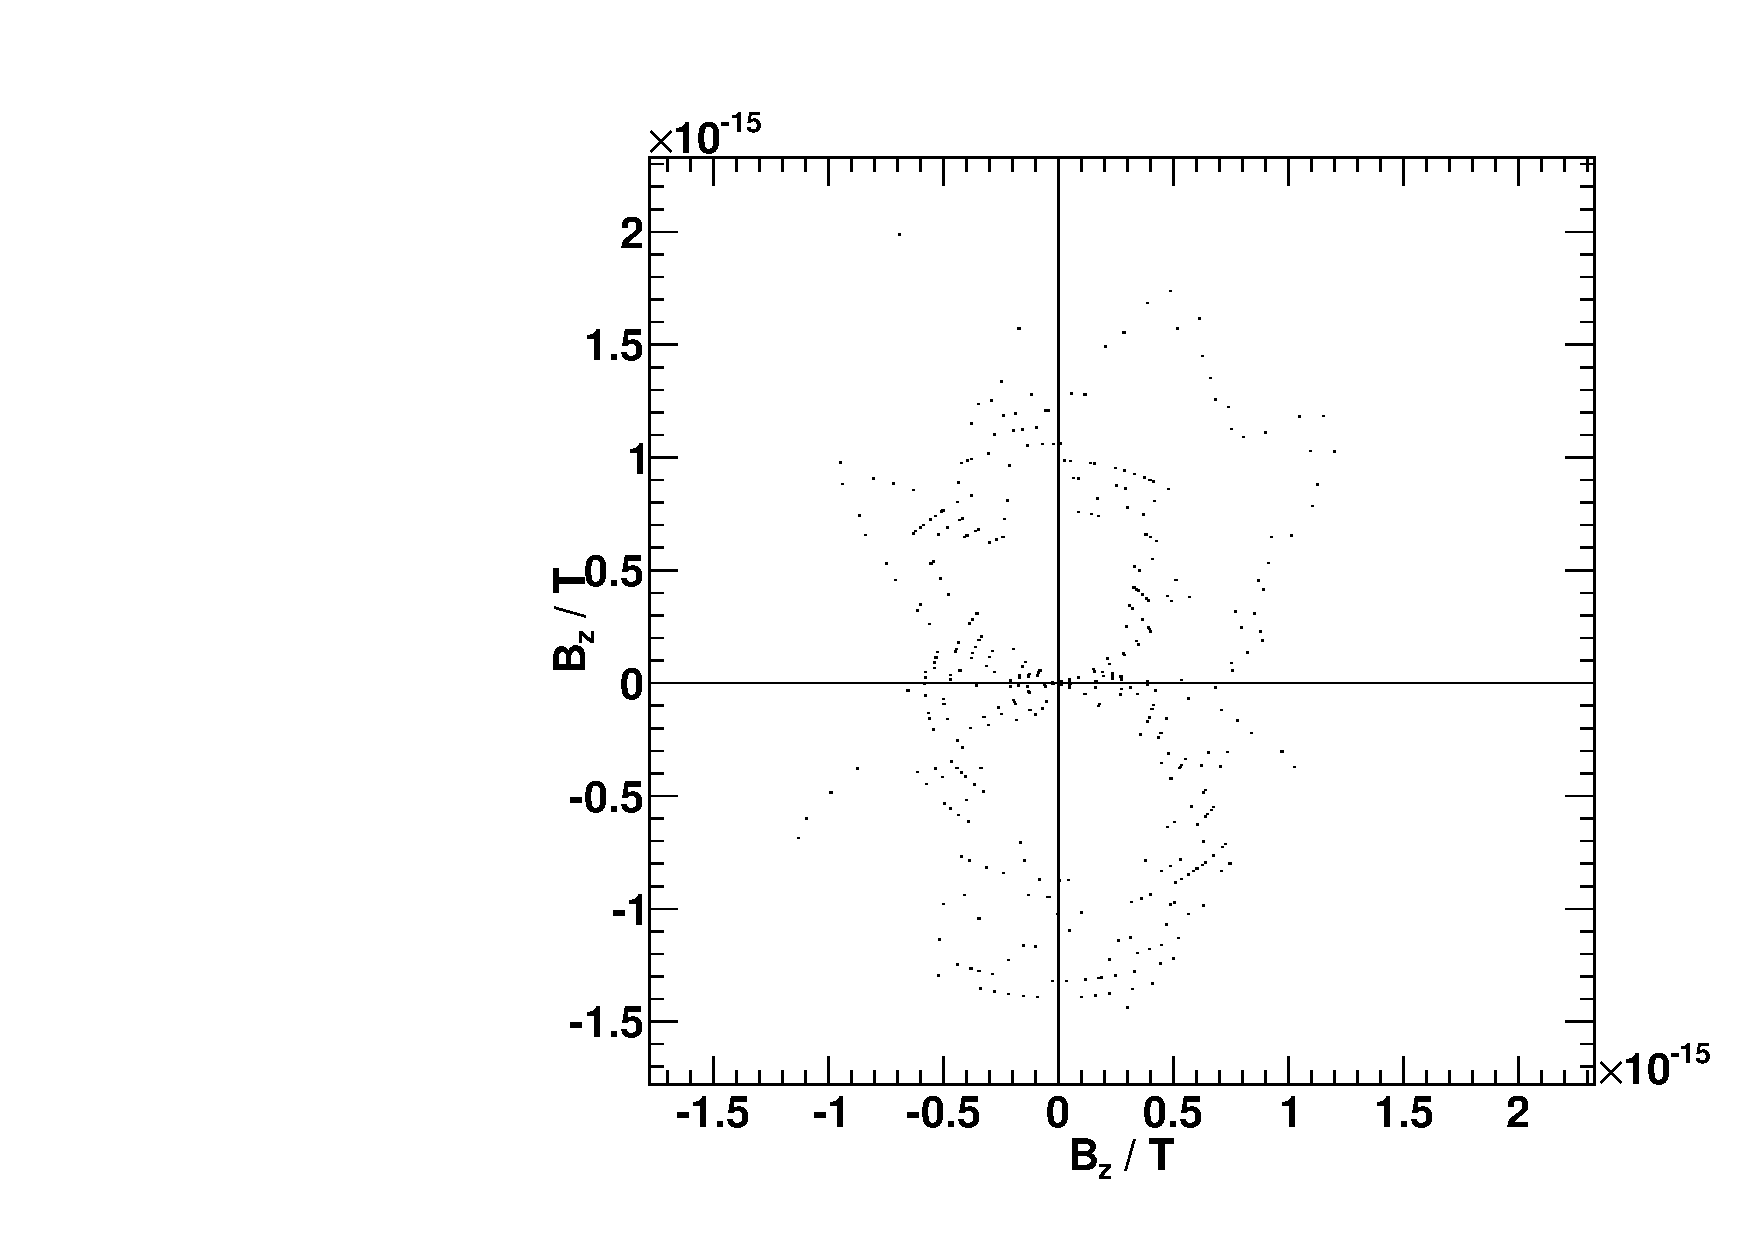
\includegraphics[width=0.35\textwidth]{../img/polar_Spule_R5_1.pdf}
  \caption{caption}
  \label{img:R5}
\end{center}
\end{figure}

\subsubsection{Berechnung aus der Geometrie der Leiterschleife}

\subsubsection{Vergleich}

\subsection{Vermessung des Magnetfelder verschiedener Proben}
\subsubsection{Untergrund}
\begin{figure}[H]
\begin{center}
  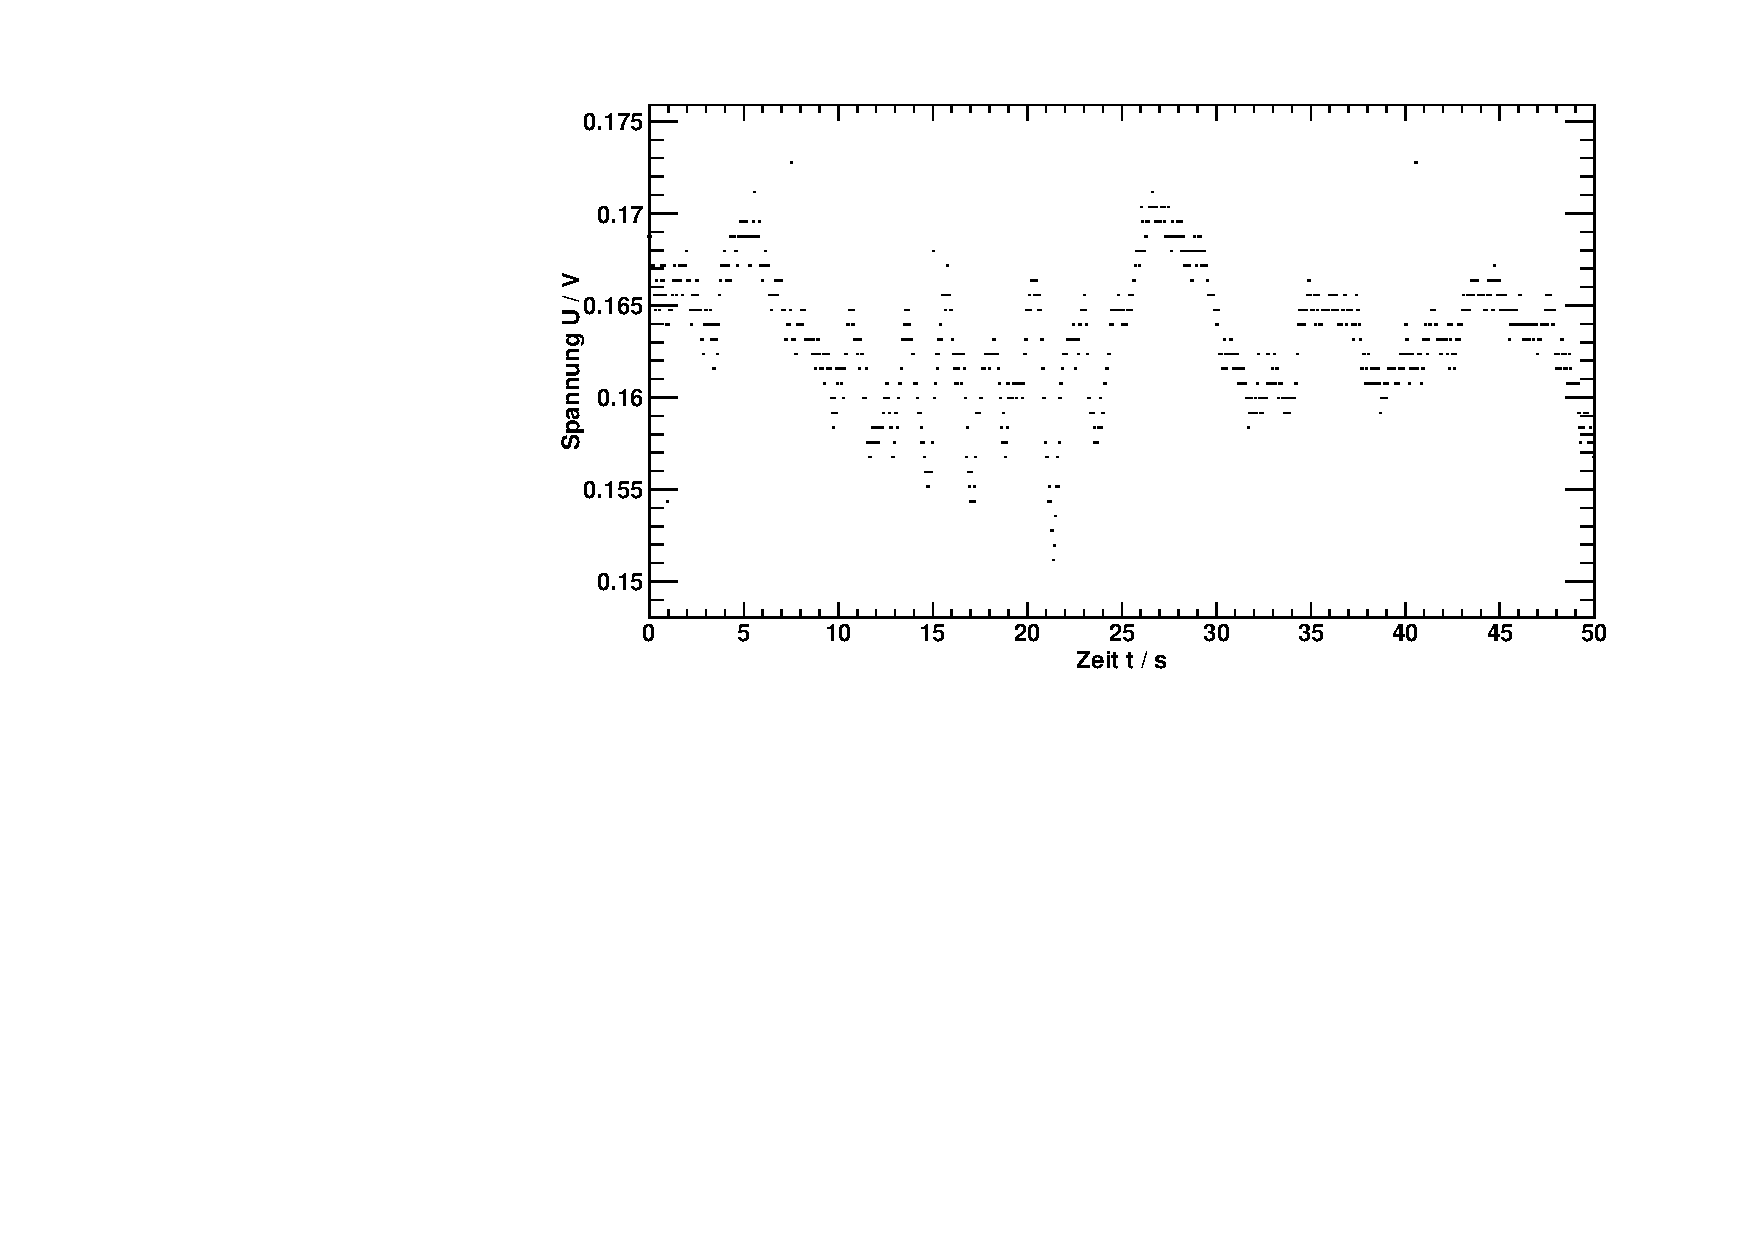
\includegraphics[width=0.64\textwidth]{../img/Untergrund.pdf}
  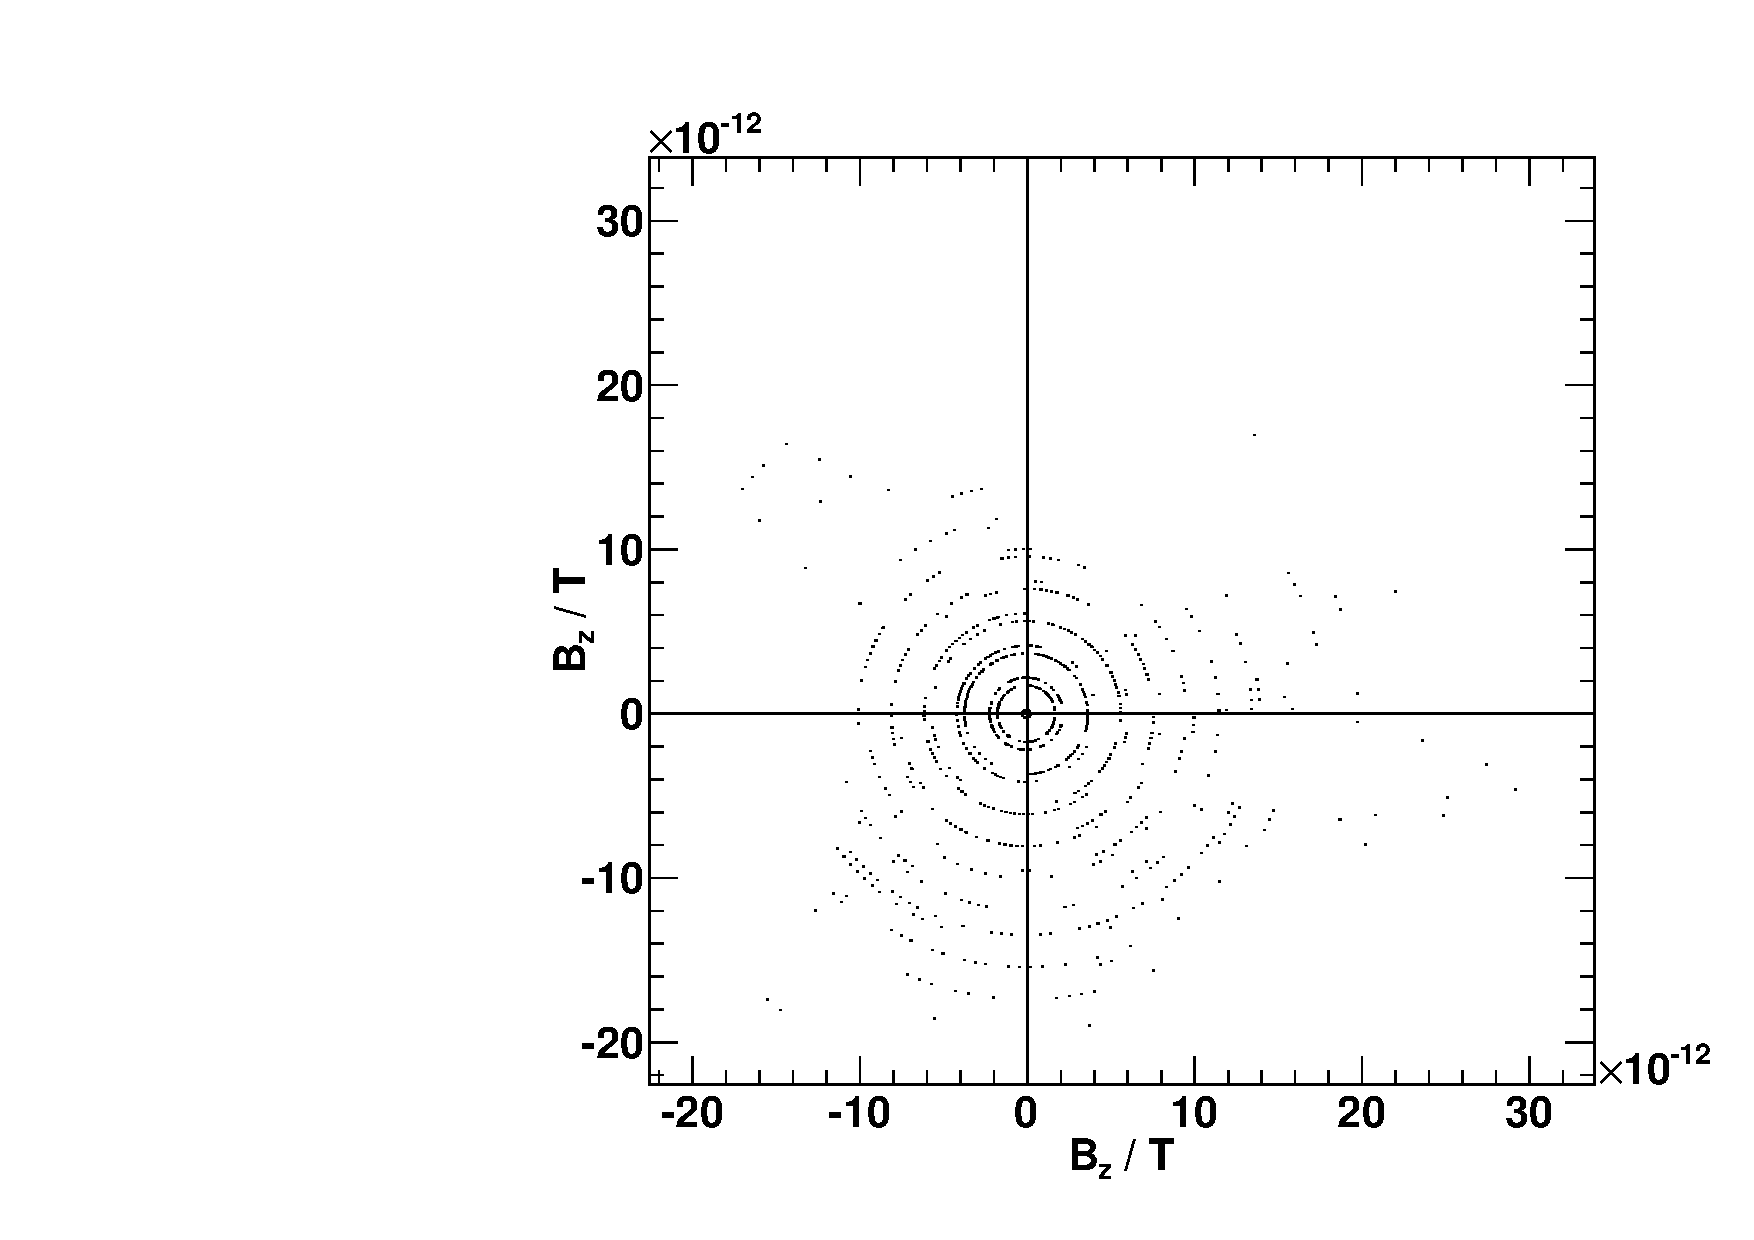
\includegraphics[width=0.35\textwidth]{../img/polar_Untergrund.pdf}
  \caption{caption}
  \label{img:underground}
\end{center}
\end{figure}

\subsubsection{Probenhalter}
\begin{figure}[H]
\begin{center}
  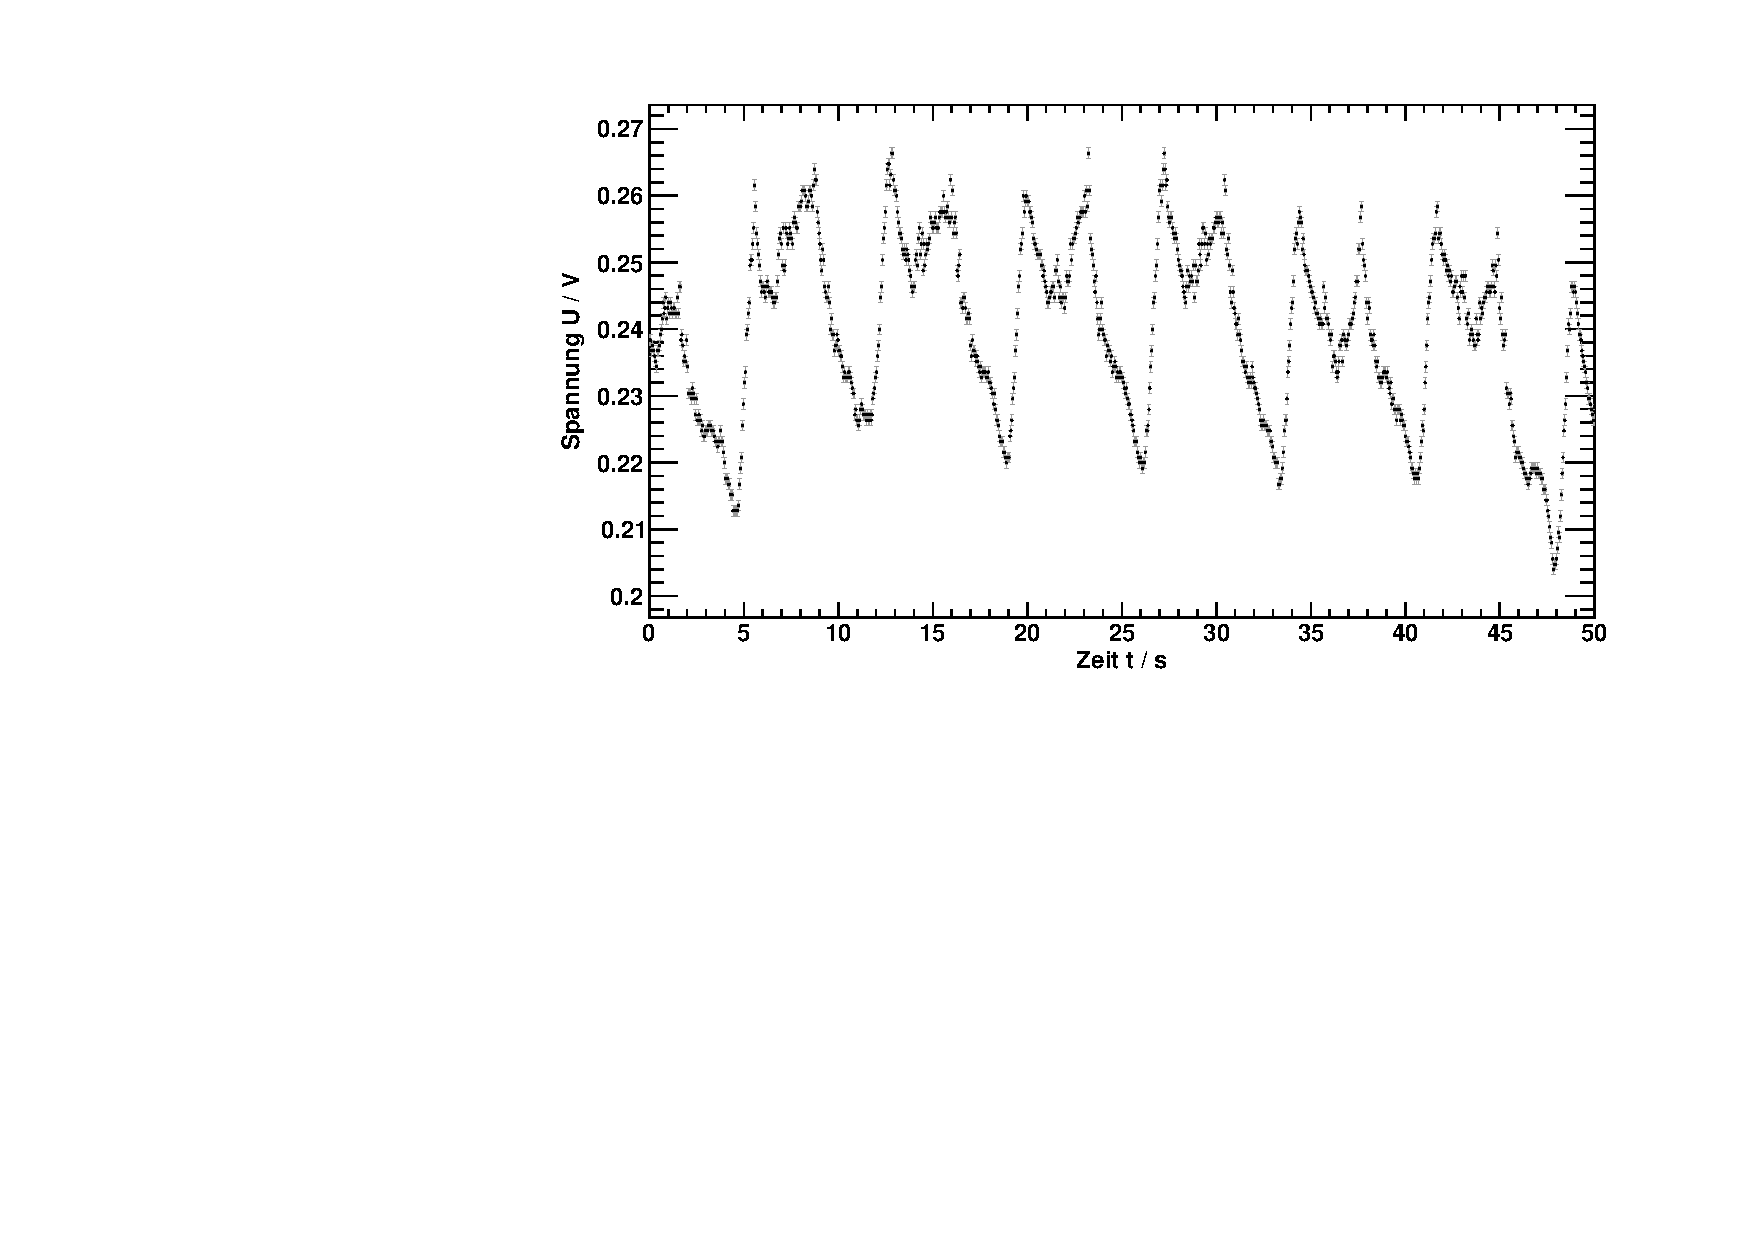
\includegraphics[width=0.64\textwidth]{../img/emptyHolder.pdf}
  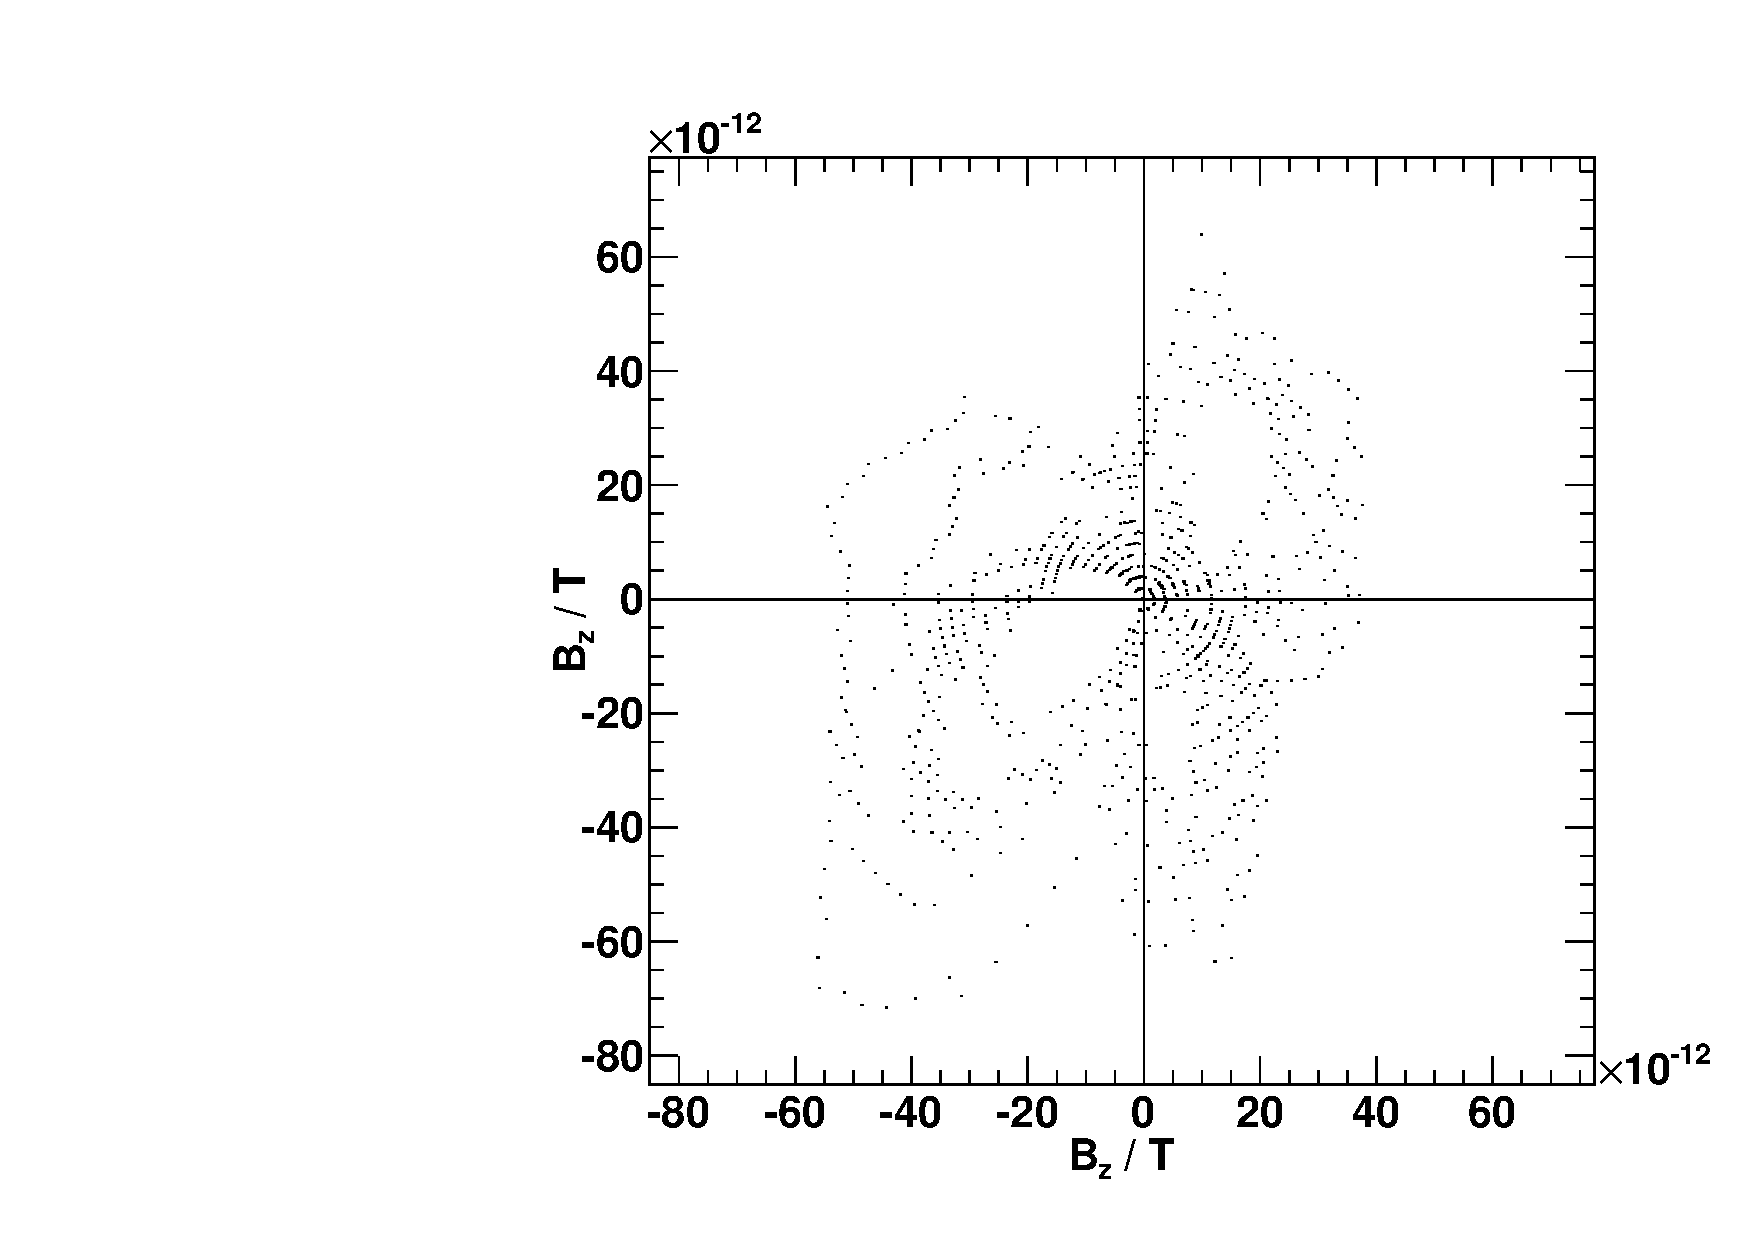
\includegraphics[width=0.35\textwidth]{../img/polar_emptyHolder.pdf}
  \caption{caption}
  \label{img:holder}
\end{center}
\end{figure}
\subsubsection{Stabmagnet}
\begin{figure}[H]
\begin{center}
  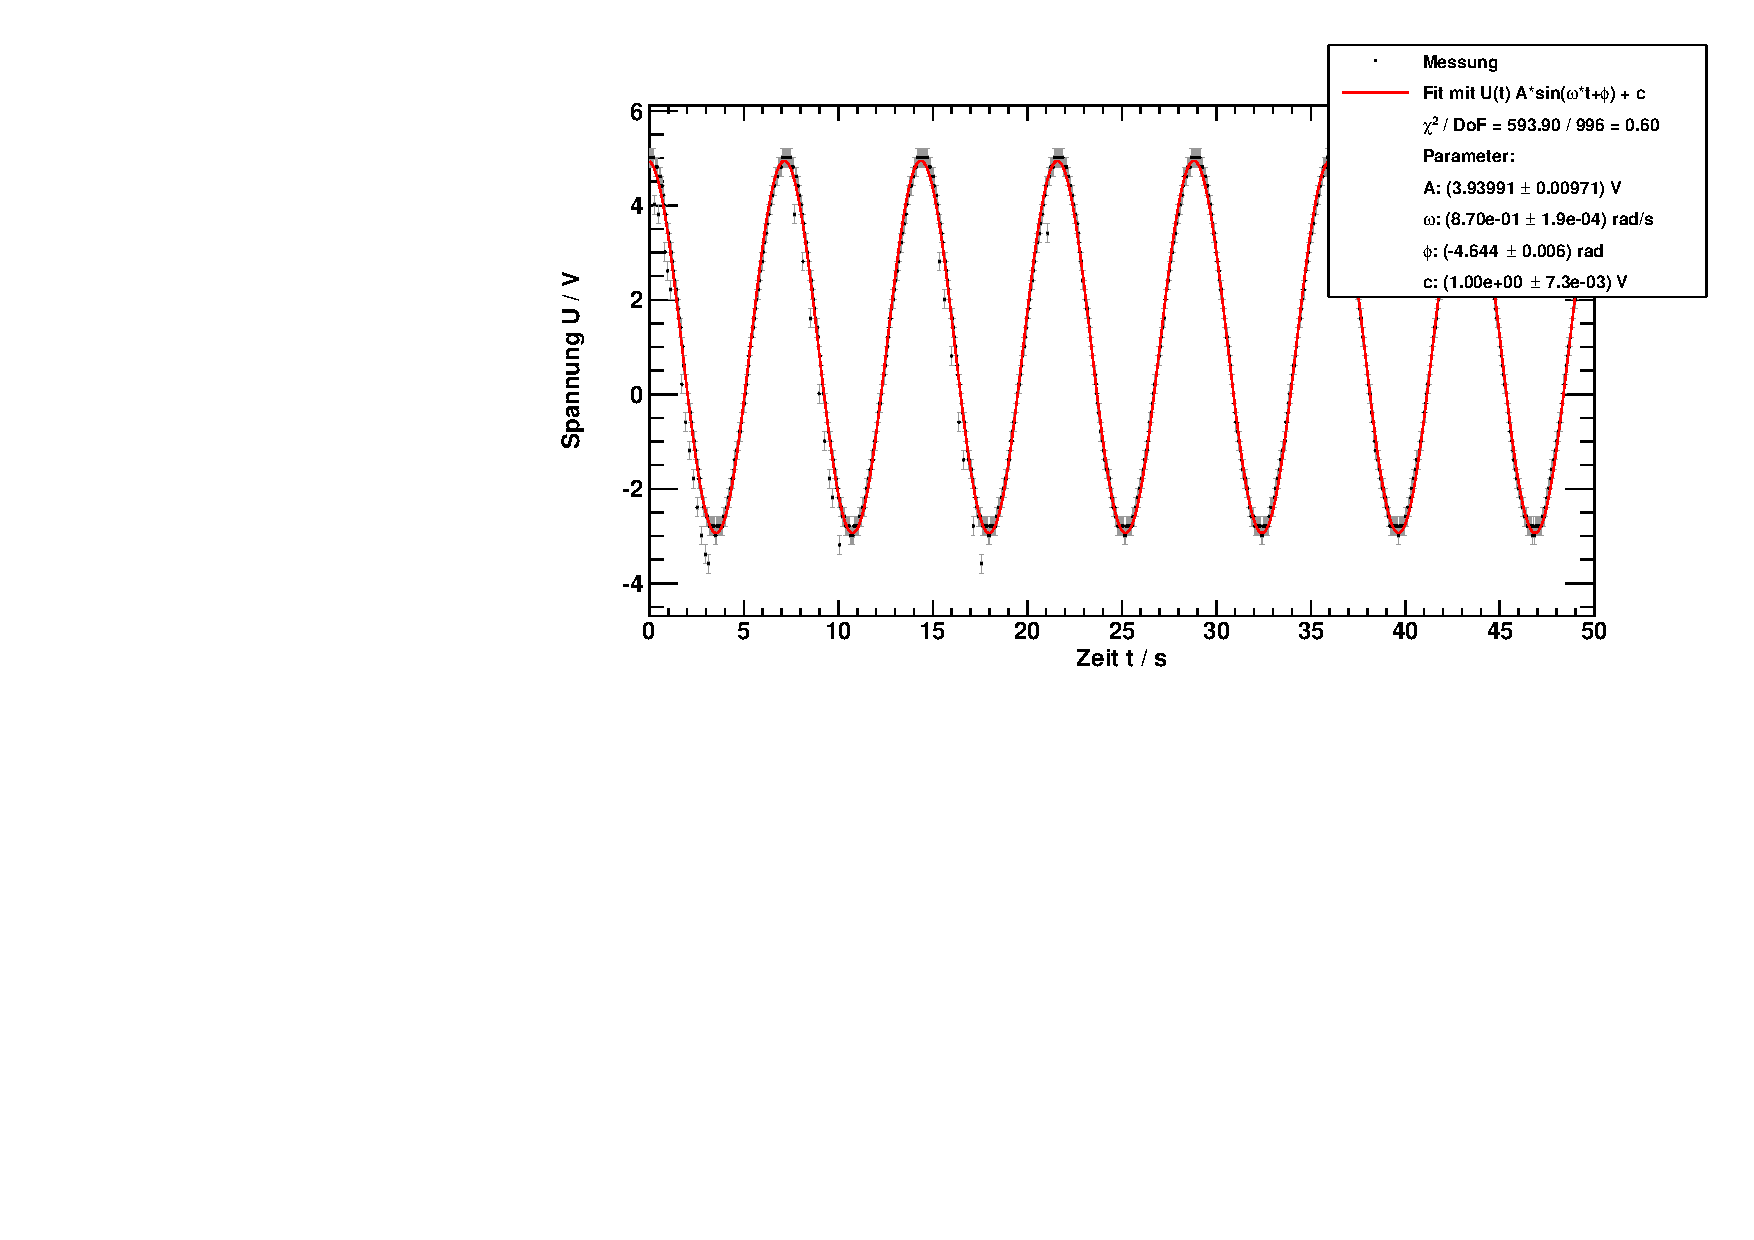
\includegraphics[width=0.64\textwidth]{../img/fit_Magnet.pdf}
  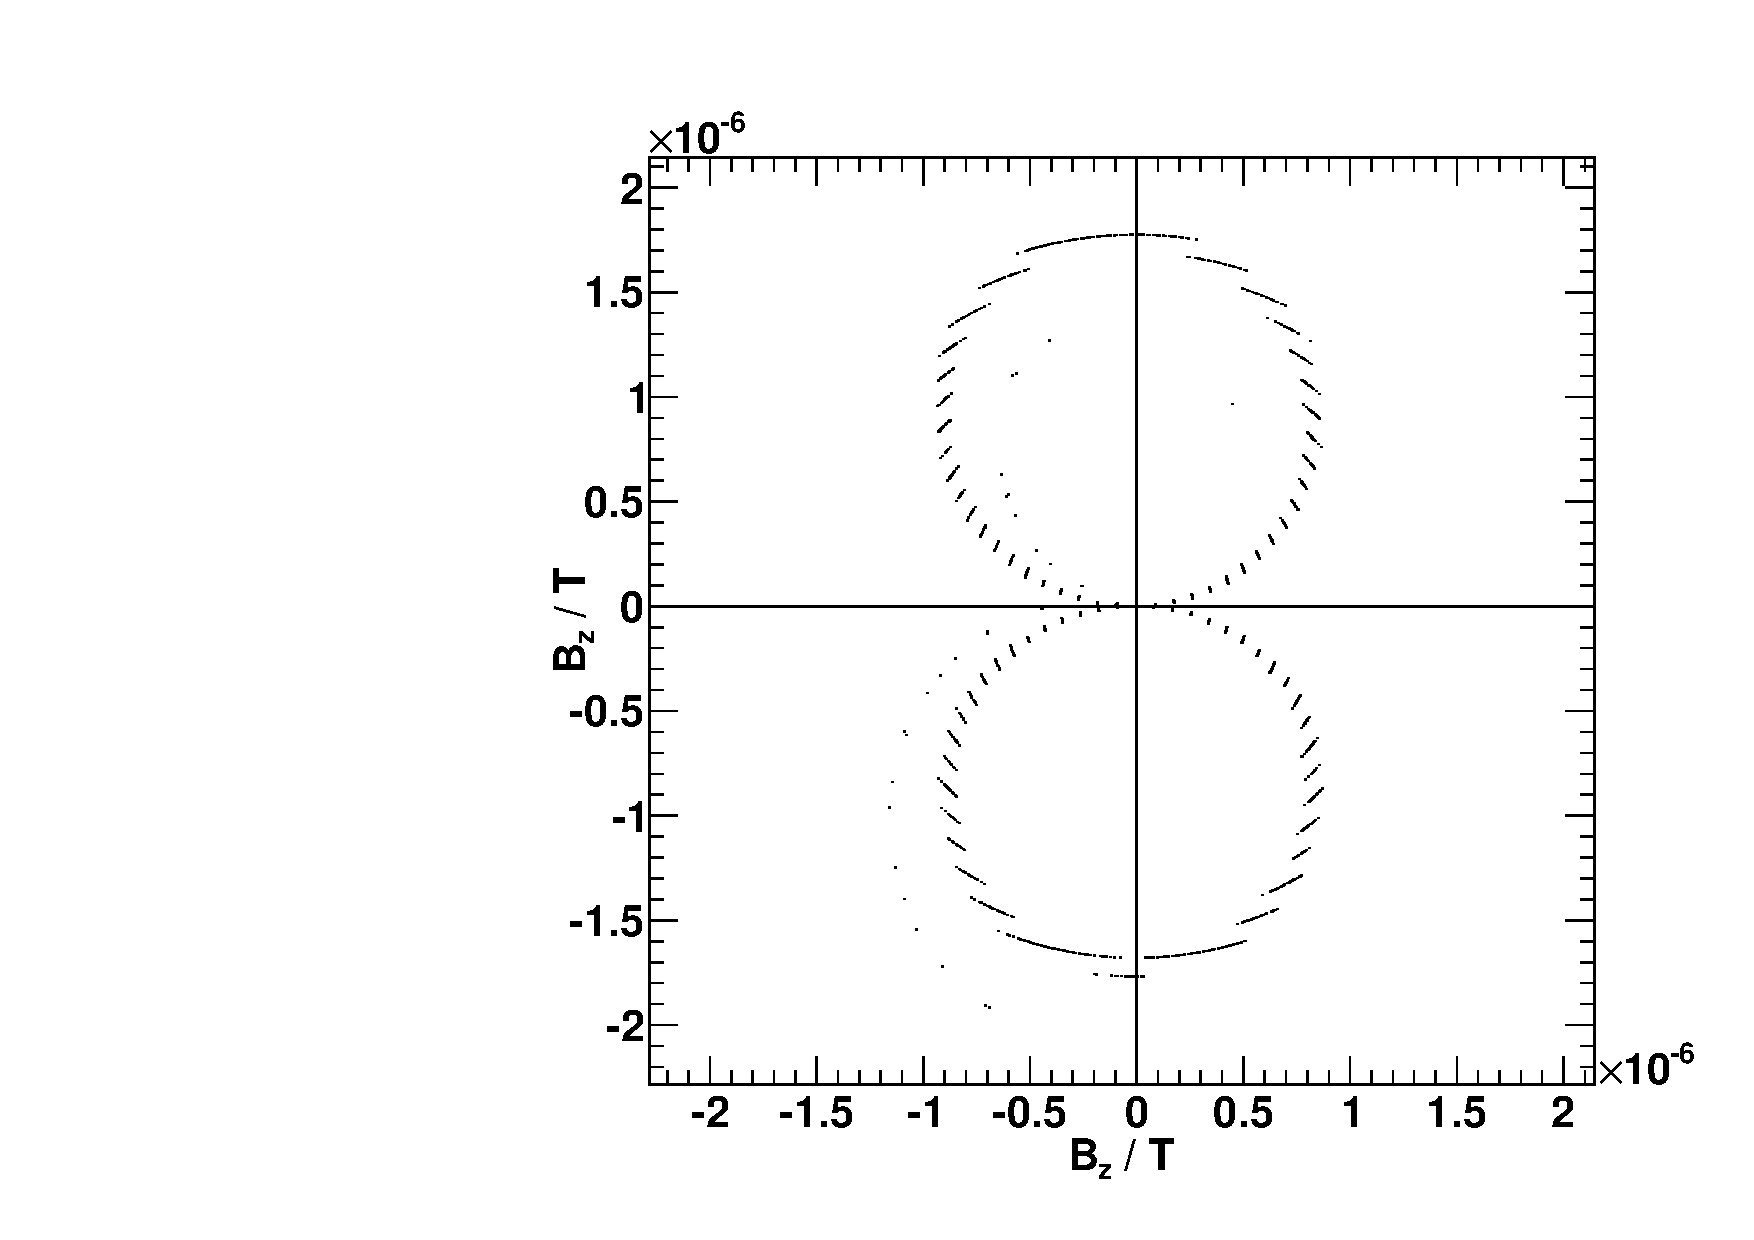
\includegraphics[width=0.35\textwidth]{../img/polar_Magnet.pdf}
  \caption{caption}
  \label{img:magnet}
\end{center}
\end{figure}

\subsubsection{Magnet-Span}
\begin{figure}[H]
\begin{center}
  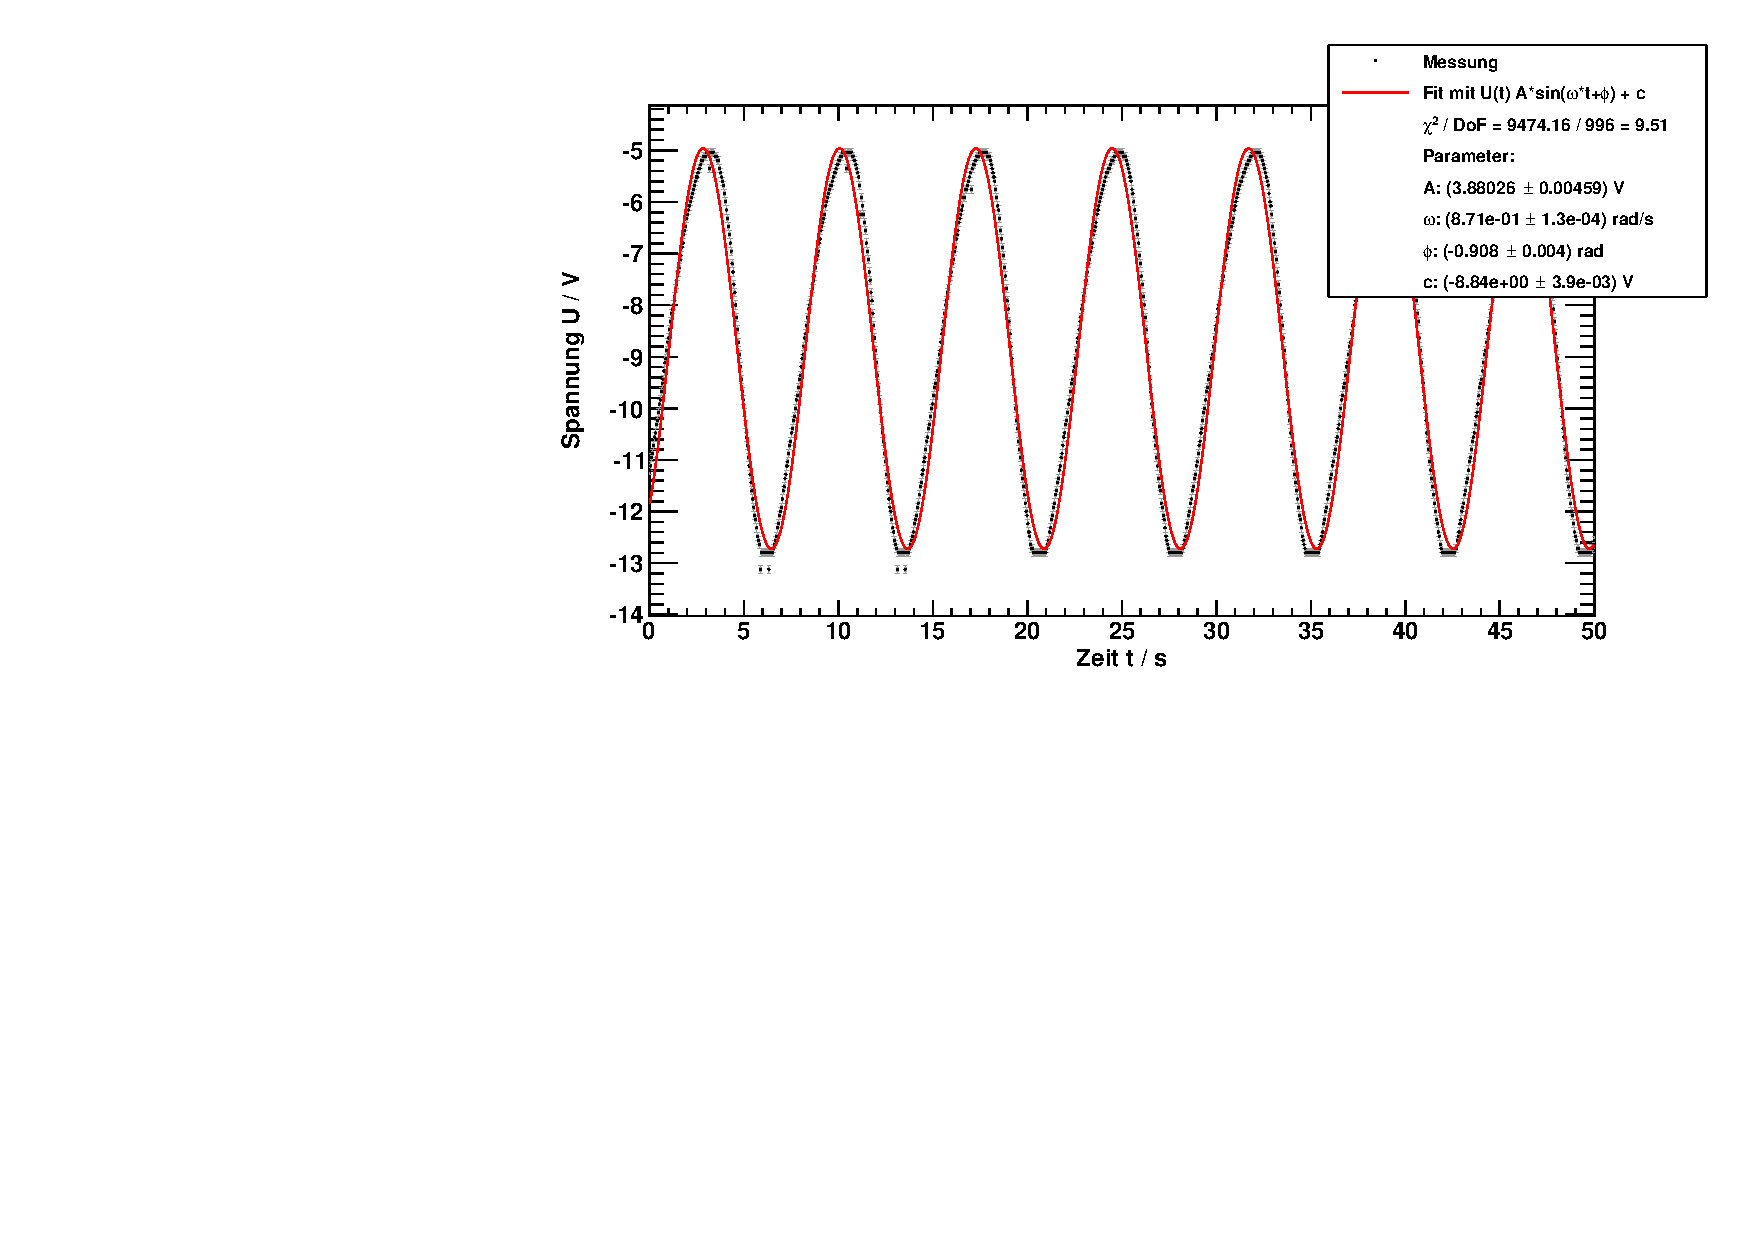
\includegraphics[width=0.64\textwidth]{../img/fit_Magnetspan_45grad.pdf}
  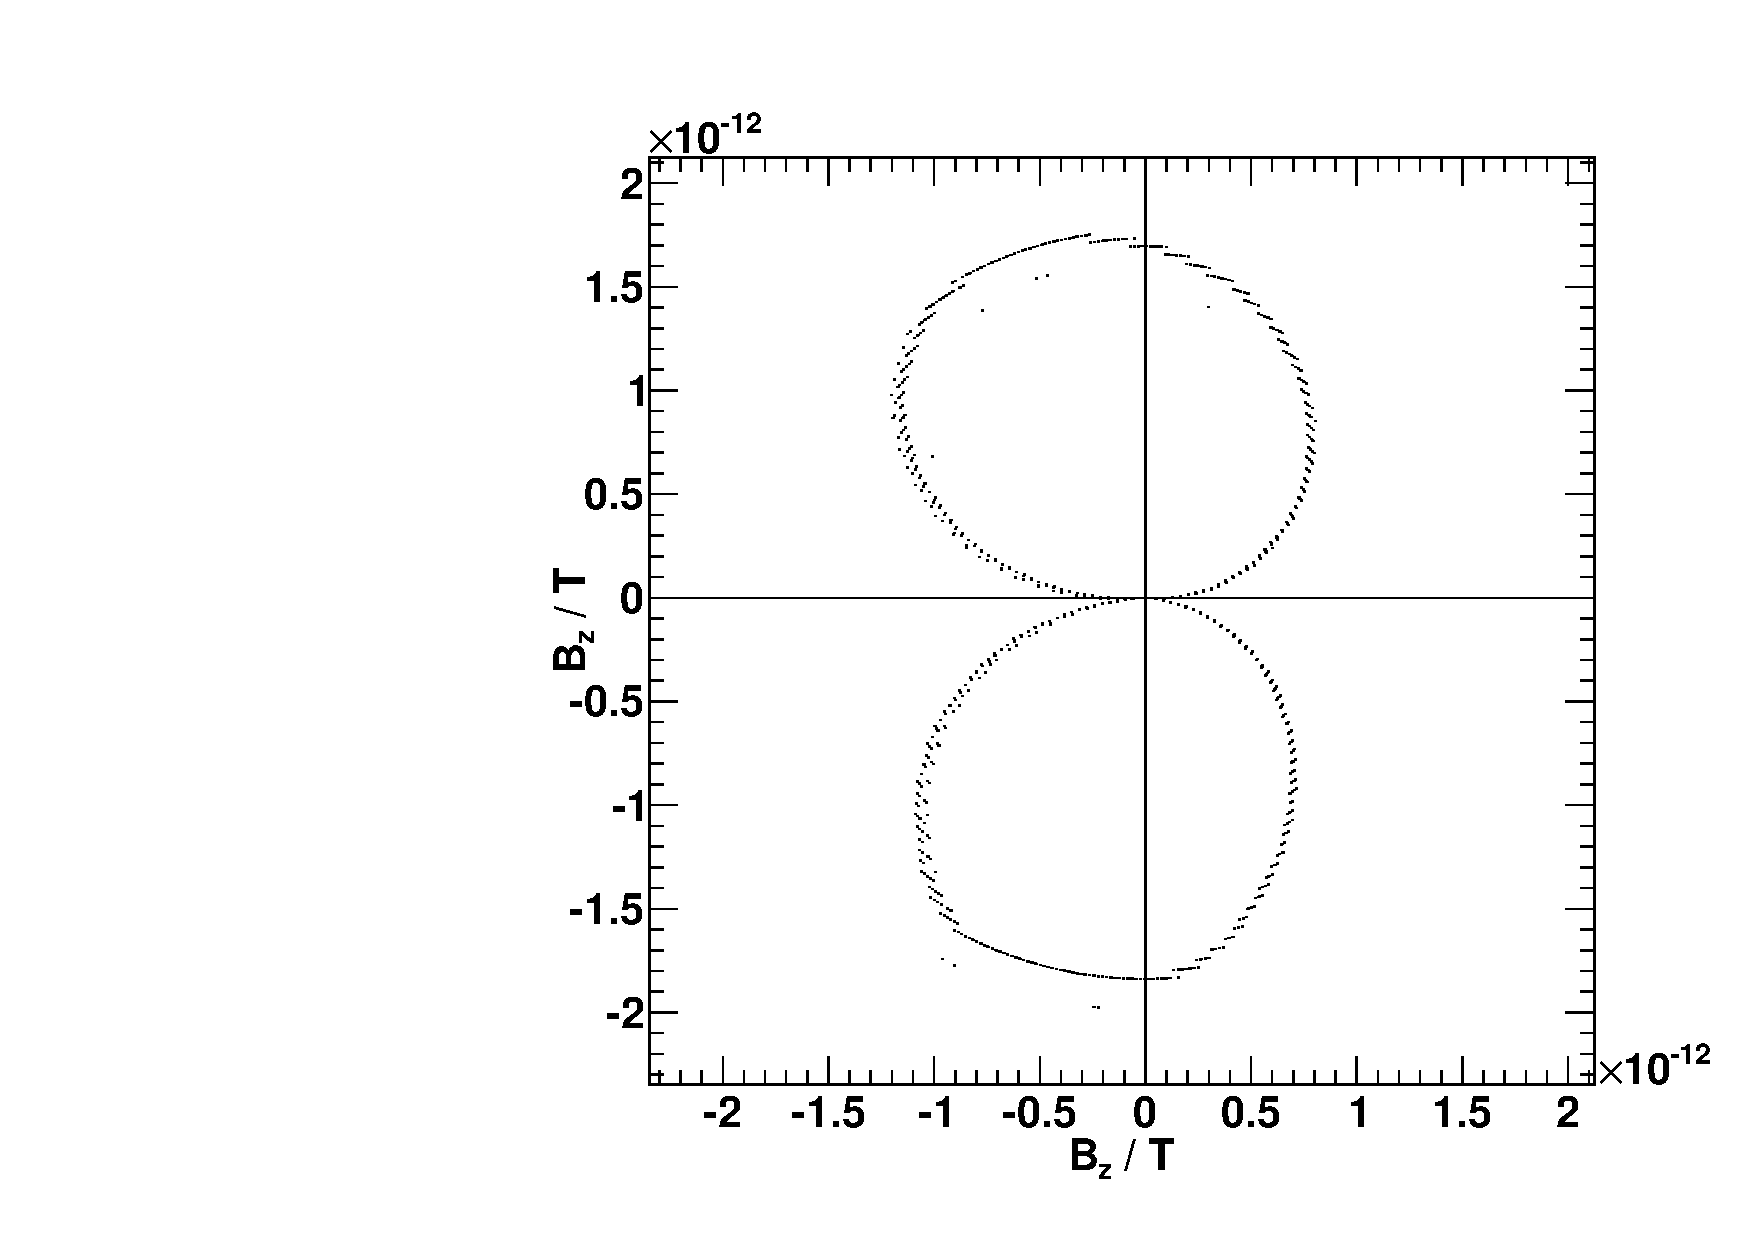
\includegraphics[width=0.35\textwidth]{../img/polar_Magnetspan_45grad.pdf}
  \caption{caption:magnetspan}
  \label{img:}
\end{center}
\end{figure}

\subsubsection{Eisen-Span}
\begin{figure}[H]
\begin{center}
  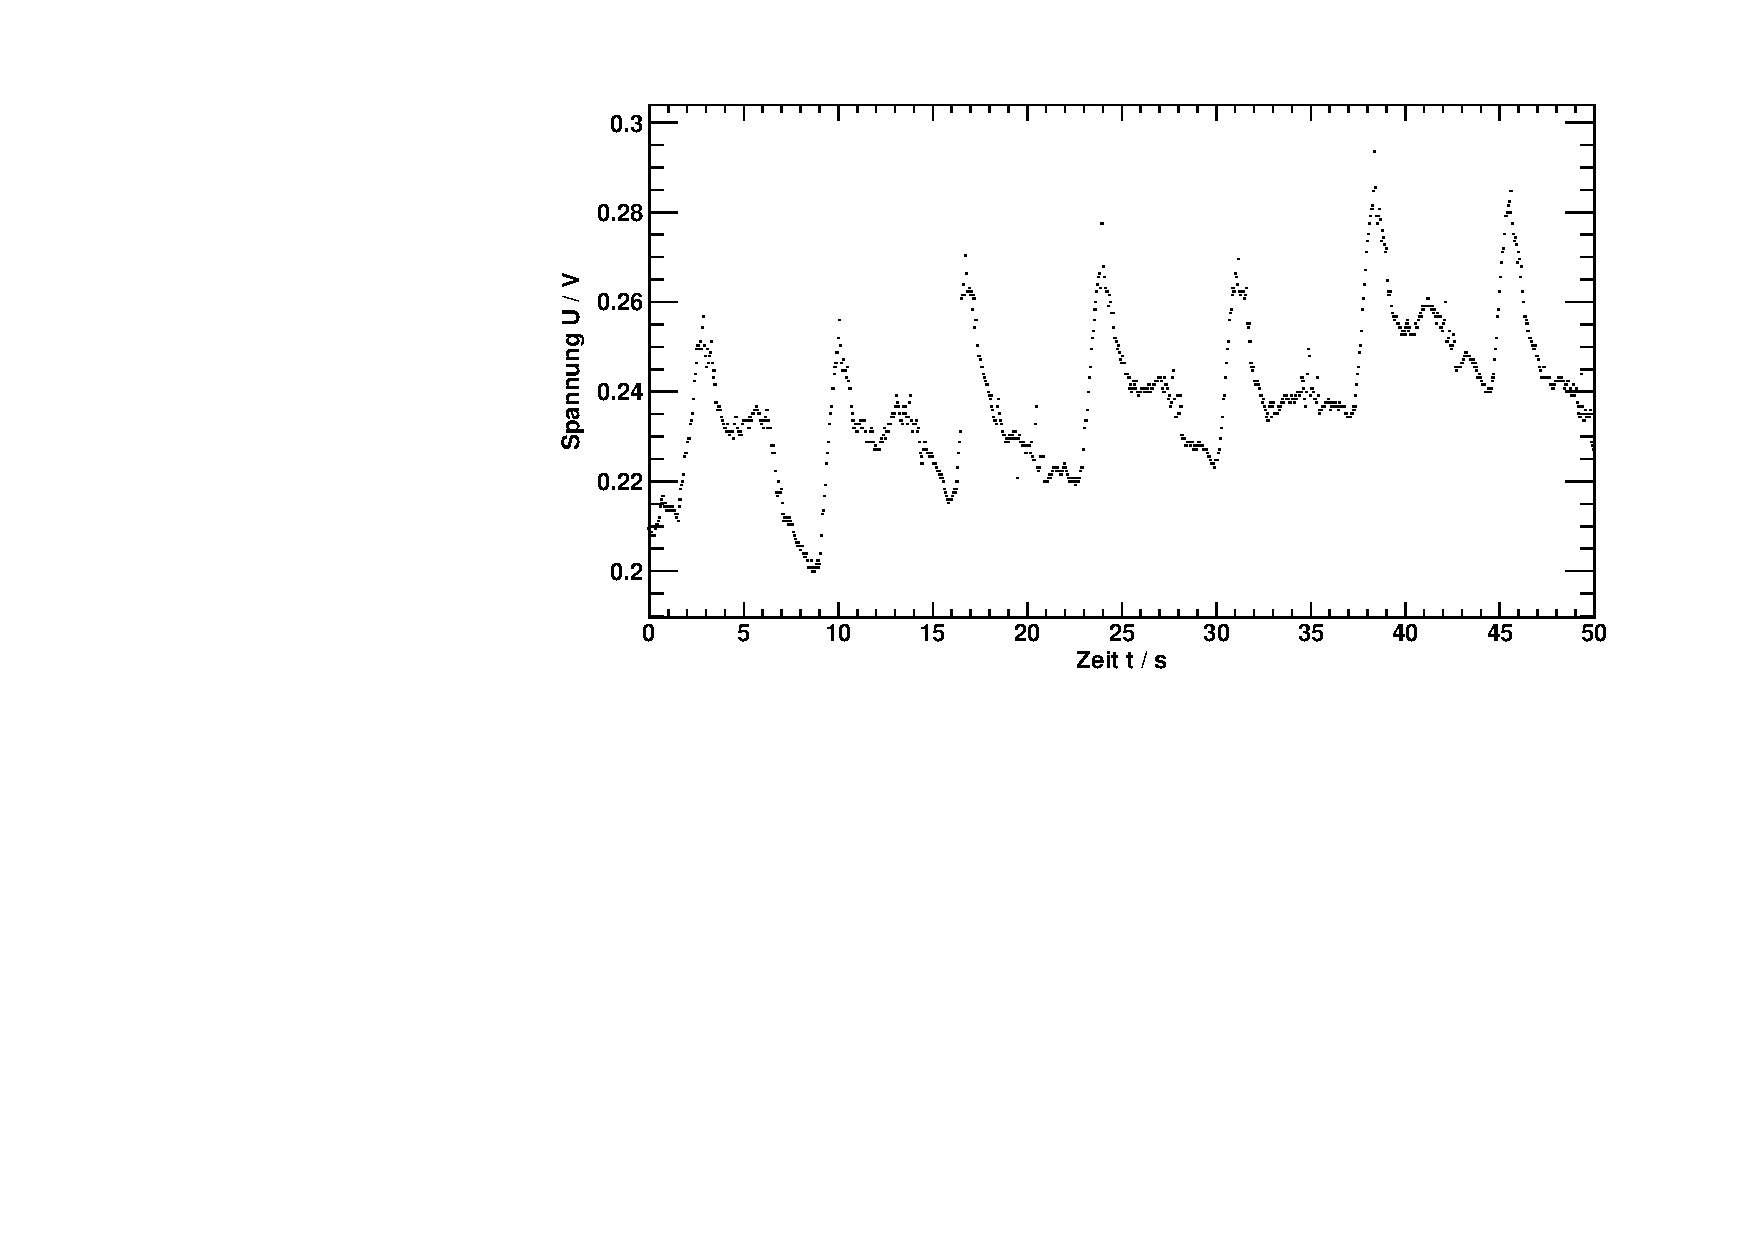
\includegraphics[width=0.64\textwidth]{../img/Fe-Span.pdf}
  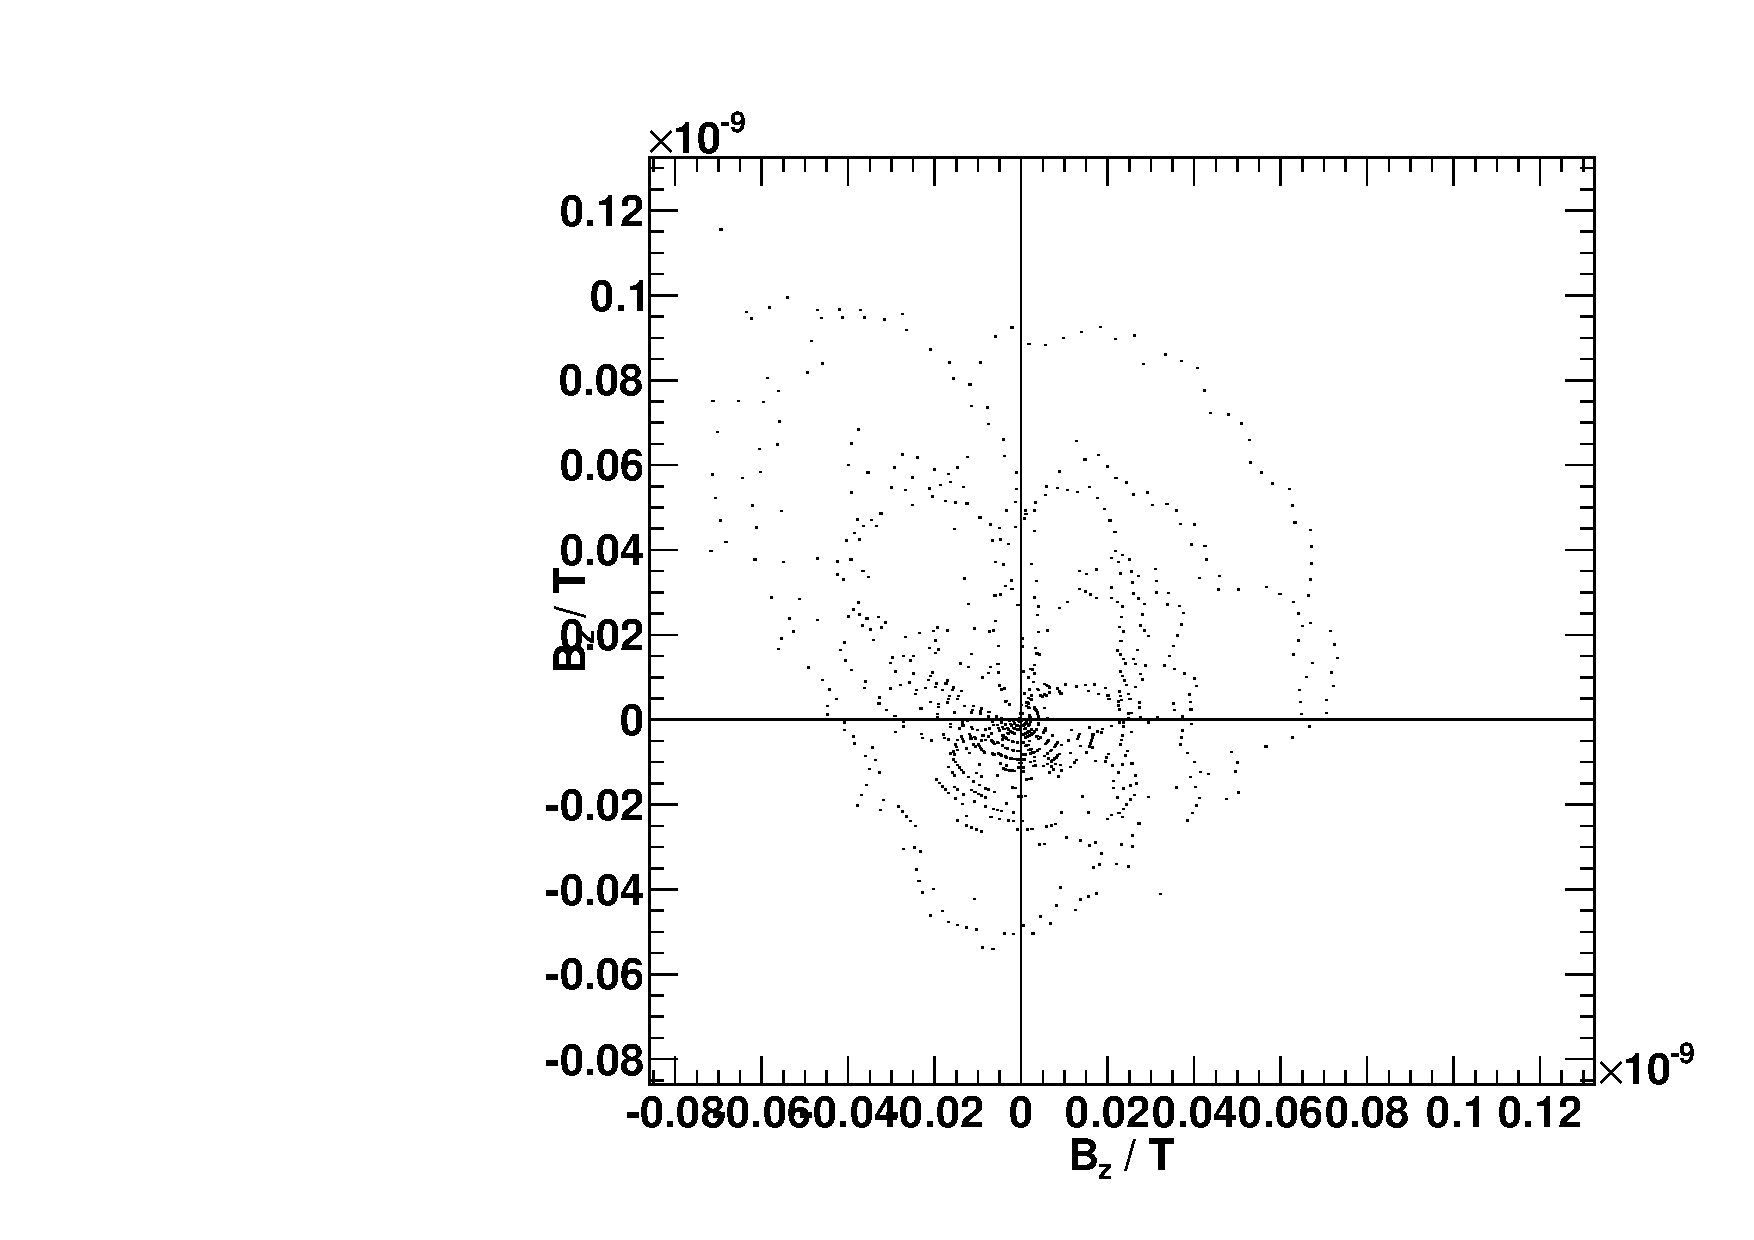
\includegraphics[width=0.35\textwidth]{../img/polar_Fe-Span.pdf}
  \caption{caption}
  \label{img:fespan}
\end{center}
\end{figure}

\subsubsection{Goldplättchen}
\begin{figure}[H]
\begin{center}
  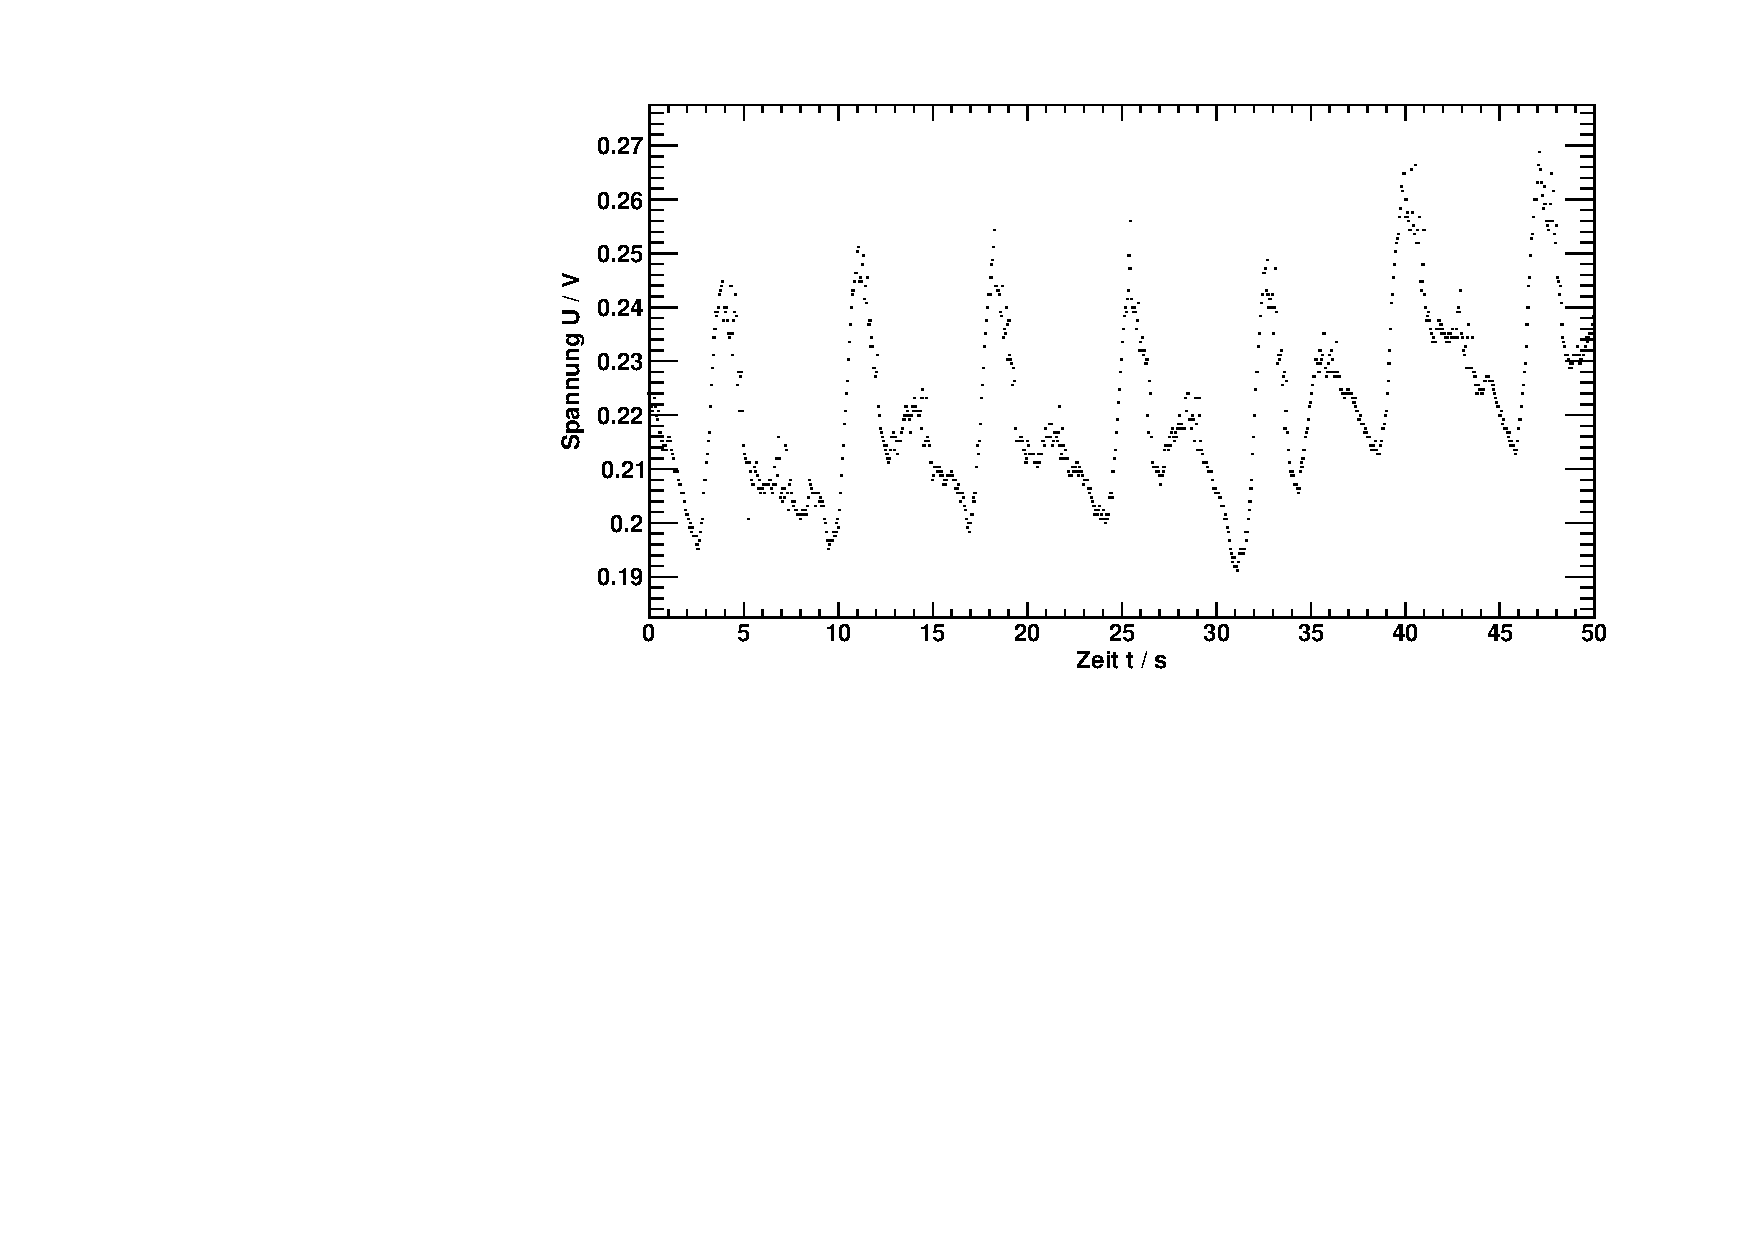
\includegraphics[width=0.64\textwidth]{../img/Au-Plaettchen.pdf}
  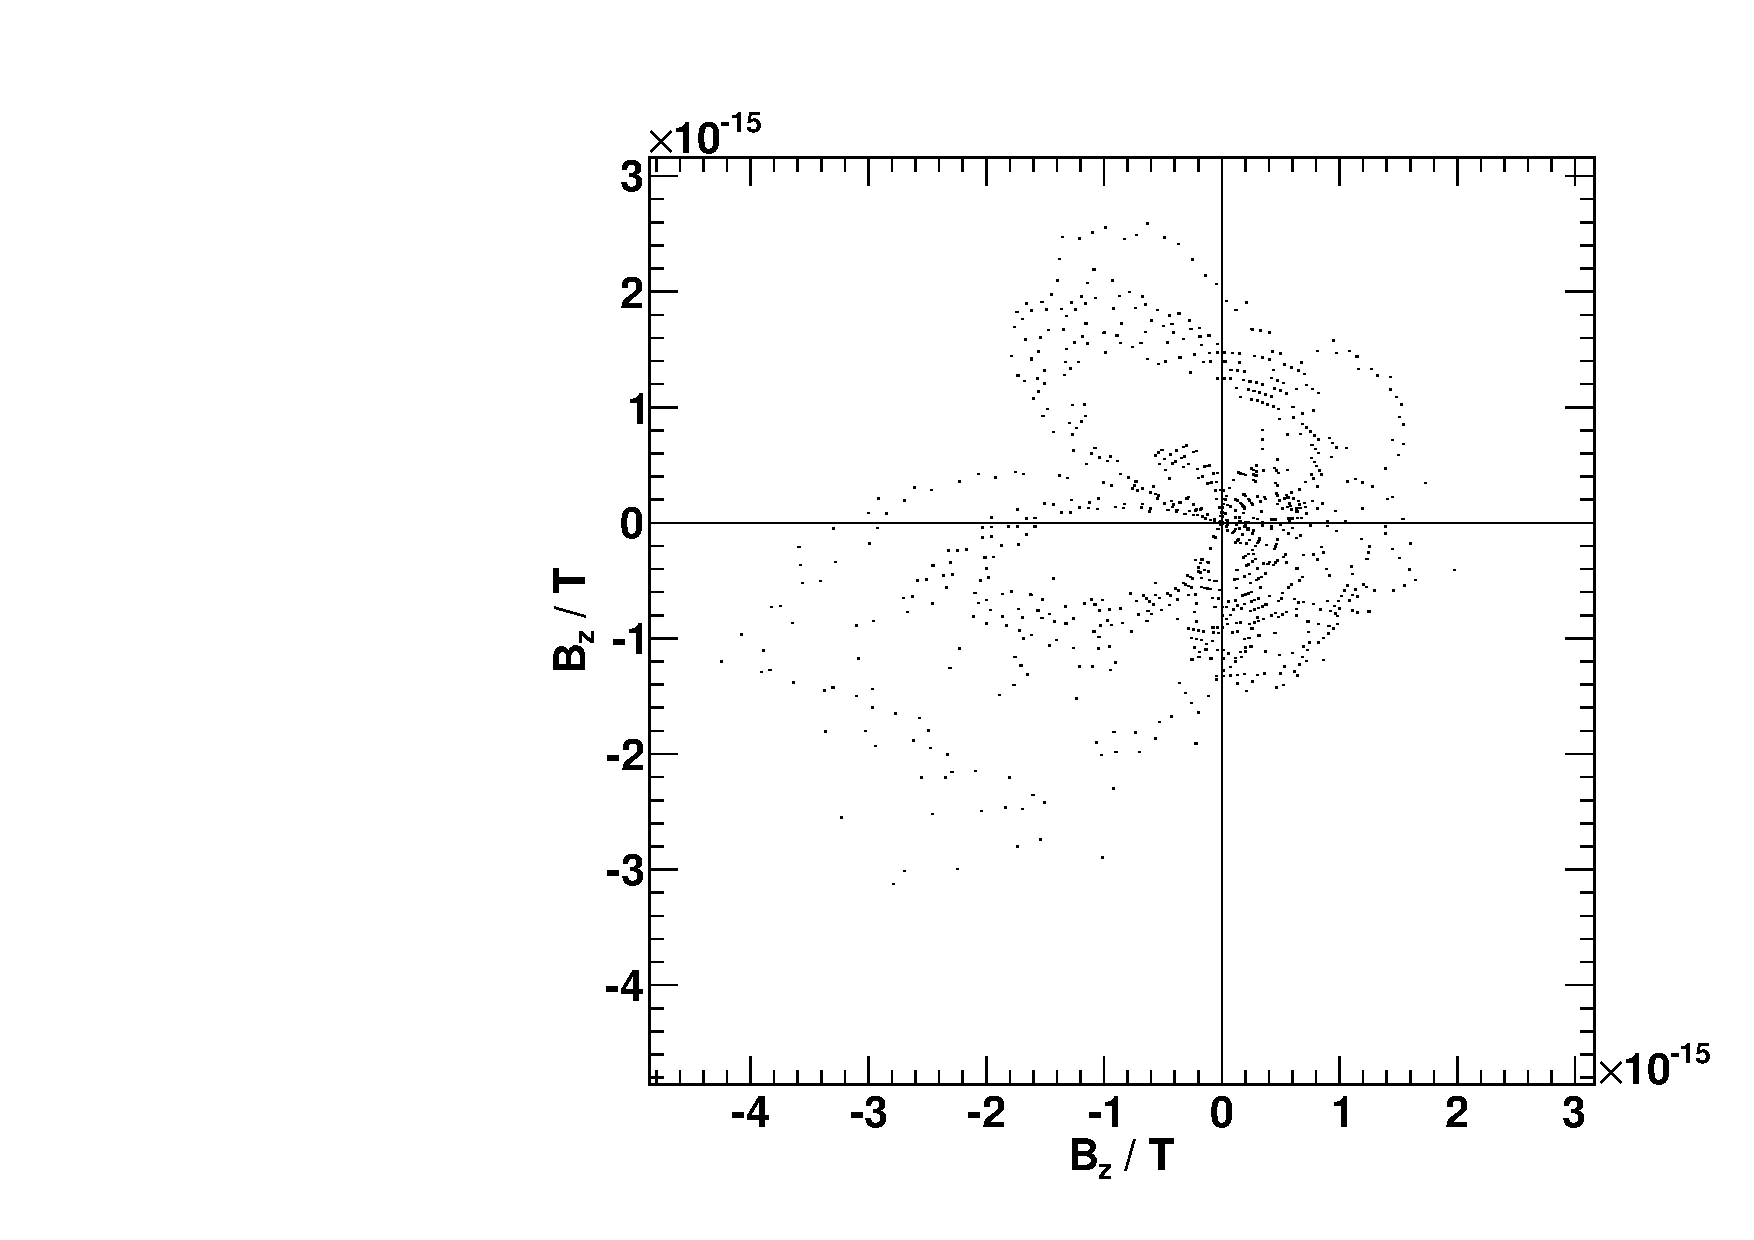
\includegraphics[width=0.35\textwidth]{../img/polar_Au-Plaettchen.pdf}
  \caption{caption}
  \label{img:au}
\end{center}
\end{figure}
